\documentclass[10pt]{article}
\usepackage[polish]{babel}
\usepackage[utf8]{inputenc}
\usepackage[T1]{fontenc}
\usepackage{amsmath}
\usepackage{amsfonts}
\usepackage{amssymb}
\usepackage[version=4]{mhchem}
\usepackage{stmaryrd}
\usepackage{graphicx}
\usepackage[export]{adjustbox}
\graphicspath{ {./images/} }
\usepackage{bbold}

%New command to display footnote whose markers will always be hidden
\let\svthefootnote\thefootnote
\newcommand\blfootnotetext[1]{%
  \let\thefootnote\relax\footnote{#1}%
  \addtocounter{footnote}{-1}%
  \let\thefootnote\svthefootnote%
}

%Overriding the \footnotetext command to hide the marker if its value is `0`
\let\svfootnotetext\footnotetext
\renewcommand\footnotetext[2][?]{%
  \if\relax#1\relax%
    \ifnum\value{footnote}=0\blfootnotetext{#2}\else\svfootnotetext{#2}\fi%
  \else%
    \if?#1\ifnum\value{footnote}=0\blfootnotetext{#2}\else\svfootnotetext{#2}\fi%
    \else\svfootnotetext[#1]{#2}\fi%
  \fi
}

\newcommand\Varangle{\mathop{{<\!\!\!\!\!\text{\small)}}\:}\nolimits}

\begin{document}
\section*{CENTRALNA \\
 KOMISJA \\
 EGZAMINACYJNA}
\begin{center}
\begin{tabular}{|l|l|}
\hline
Rodzaj dokumentu: & \begin{tabular}{l}
Zasady Oceniania rozwiązań \\
zadań \\
\end{tabular} \\
\hline
Egzamin: & Egzamin maturalny \\
\hline
Przedmiot: & Matematyka \\
\hline
Poziom: & Poziom rozszerzony \\
\hline
Formy arkusza: & \begin{tabular}{l}
EMAP-R0-100, EMAP-R0-200, \\
EMAP-R0-300, EMAP-R0-400,, \\
EMAP-R0-Q00, EMAP-R0-700, EMAP-R0-Z00,, \\
EMAU-R0-100 \\
\end{tabular} \\
\hline
Termin egzaminu: & 12 maja 2023 r. \\
\hline
\begin{tabular}{l}
Data publikacji \\
dokumentu: \\
\end{tabular} & 28 czerwca 2023 r. \\
\hline
\end{tabular}
\end{center}

\section*{ZADANIA ZAMKNIĘTE}
Zadanie 1. (0-1)

\begin{center}
\begin{tabular}{|l|l|}
\hline
\multicolumn{2}{|c|}{Wymagania egzaminacyjne 2023 i 2024 $^{1}$} \\
\hline
\multicolumn{1}{|c|}{Wymaganie ogólne} & \multicolumn{1}{c|}{Wymaganie szczegółowe} \\
\hline
I. Wykorzystanie i tworzenie informacji. & Zdający: \\
 & R11.1) oblicza granice funkcji (i granice \\
 & jednostronne), korzystając z twierdzeń \\
 & \begin{tabular}{l}
odziałaniach na granicach i z własności \\
funkcji ciągłych. \\
\end{tabular} \\
\hline
\end{tabular}
\end{center}

\section*{Zasady oceniania}
1 pkt - odpowiedź poprawna.\\
0 pkt - odpowiedź niepoprawna albo brak odpowiedzi.

\section*{Rozwiązanie}
D

\section*{Zadanie 2. (0-1)}
\begin{center}
\begin{tabular}{|l|l|}
\hline
\multicolumn{2}{|c|}{Wymagania egzaminacyjne 2023 i 2024} \\
\hline
\multicolumn{1}{|c|}{Wymaganie ogólne} & \multicolumn{1}{c|}{Wymaganie szczegółowe} \\
\hline
II. Wykorzystanie i interpretowanie & Zdający: \\
reprezentacji. & R8.4) oblicza współrzędne oraz długość \\
 & wektora; dodaje i odejmuje wektory oraz \\
 & mnoży je przez liczbę. Interpretuje \\
 & geometrycznie działania na wektorach. \\
\hline
\end{tabular}
\end{center}

\section*{Zasady oceniania}
1 pkt - odpowiedź poprawna.\\
0 pkt - odpowiedź niepoprawna albo brak odpowiedzi.

\section*{Rozwiązanie}
C

\footnotetext{${ }^{1}$ Rozporządzenie Ministra Edukacji i Nauki z dnia 1 sierpnia 2022 r. w sprawie wymagań egzaminacyjnych dla egzaminu maturalnego przeprowadzanego w roku szkolnym 2022/2023 i 2023/2024 (Dz.U. poz. 1698).
}Zadanie 3. (0-1)

\begin{center}
\begin{tabular}{|l|l|}
\hline
\multicolumn{2}{|c|}{Wymagania egzaminacyjne 2023 i 2024} \\
\hline
\multicolumn{1}{|c|}{Wymaganie ogólne} & \multicolumn{1}{c|}{Wymaganie szczegółowe} \\
\hline
IV. Użycie i tworzenie strategii. & Zdający: \\
 & R7.1) stosuje twierdzenia charakteryzujące \\
 & \begin{tabular}{l}
czworokąty wpisane w okrąg i czworokąty \\
opisane na okręgu. \\
\hline
\end{tabular} \\
\hline
\end{tabular}
\end{center}

\section*{Zasady oceniania}
1 pkt - odpowiedź poprawna.\\
0 pkt - odpowiedź niepoprawna albo brak odpowiedzi.

\section*{Rozwiązanie}
B

\section*{Zadanie 4. (0-1)}
\begin{center}
\begin{tabular}{|l|l|}
\hline
\multicolumn{2}{|c|}{Wymagania egzaminacyjne 2023 i 2024} \\
\hline
\multicolumn{1}{|c|}{Wymaganie ogólne} & \multicolumn{1}{|c|}{Wymaganie szczegółowe} \\
\hline
III. Modelowanie matematyczne. & Zdający: \\
 & R10.1) wykorzystuje wzory na liczbe \\
 & permutacji, kombinacji, wariacji i wariacji \\
 & z powtórzeniami do zliczania obiektów \\
 & w sytuacjach kombinatorycznych. \\
\hline
\end{tabular}
\end{center}

\section*{Zasady oceniania}
1 pkt - odpowiedź poprawna.\\
0 pkt - odpowiedź niepoprawna albo brak odpowiedzi.

\section*{Rozwiązanie}
C

\section*{Zadanie otwarte (kodowane)}
\section*{Zadanie 5. (0-2)}
\begin{center}
\begin{tabular}{|l|l|}
\hline
\multicolumn{2}{|c|}{Wymagania egzaminacyjne 2023 i 2024} \\
\hline
\multicolumn{1}{|c|}{Wymaganie ogólne} & \multicolumn{1}{c|}{Wymaganie szczegółowe} \\
\hline
\begin{tabular}{ll}
II. Wykorzystanie i interpretowanie &  \\
reprezentacji. & \begin{tabular}{l}
Zdajacy: \\
R3.5) stosuje twierdzenie o pierwiastkach \\
wymiernych wielomianu o współczynnikach \\
całkowitych. \\
\end{tabular} \\
\hline
\end{tabular} &  \\
\hline
\end{tabular}
\end{center}

\section*{Zasady oceniania}
2 pkt - odpowiedź całkowicie poprawna.\\
0 pkt - odpowiedź niepełna lub niepoprawna albo brak odpowiedzi.

\section*{Rozwiązanie}
\begin{center}
\begin{tabular}{|l|l|l|}
\hline
2 & 8 & 5 \\
\hline
\end{tabular}
\end{center}

\section*{Zadania otwarte (niekodowane)}
\section*{Uwagi ogólne:}
\begin{enumerate}
  \item Akceptowane są wszystkie rozwiązania merytorycznie poprawne i spełniające warunki zadania
  \item Jeżeli zdający popełni błędy rachunkowe, które na żadnym etapie rozwiązania nie upraszczają i nie zmieniają danego zagadnienia, lecz stosuje poprawną metodę i konsekwentnie do popełnionych błędów rachunkowych rozwiązuje zadanie, to może otrzymać co najwyżej ( $n-1$ ) punktów (gdzie $n$ jest maksymalną możliwą do uzyskania liczbą punktów za dane zadanie).
\end{enumerate}

\section*{Zadanie 6. (0-3)}
\begin{center}
\begin{tabular}{|l|l|}
\hline
\multicolumn{2}{|c|}{Wymagania egzaminacyjne 2023 i 2024} \\
\hline
\multicolumn{1}{|c|}{Wymaganie ogólne} & \multicolumn{1}{|c|}{Wymaganie szczegółowe} \\
\hline
V. Rozumowanie i argumentacja. & Zdajacy: \\
 & \begin{tabular}{l}
R2.1) używa wzorów skróconego mnożenia \\
 \\
 \\
 \\
 \\
\end{tabular}$|$\begin{tabular}{l}
na $(a \pm b)^{3}$ oraz $a^{3} \pm b^{3}$. \\
\hline
\end{tabular} \\
\hline
\end{tabular}
\end{center}

\section*{Zasady oceniania}
3 pkt - przeprowadzenie pełnego rozumowania, tj. przekształcenie nierówności $x^{3}-x^{2} y \leq x y^{2}-y^{3}$ do postaci, z której można bezpośrednio wnioskować o równości liczb $x$ i $y$ (lub do postaci, z której można bezpośrednio wnioskować, że jedna $z$ liczb: $x, y$, jest równa 2 ) oraz obliczenie tych liczb: $x=2$ oraz $y=2$.

2 pkt - zastosowanie wzoru na sześcian różnicy oraz kwadrat różnicy, wykorzystanie założenia i zapisanie nierówności kwadratowej $z$ jedną niewiadomą $x$ (lub $y$ ) w postaci $a x^{2}+b x+c \geq 0$ lub $a x^{2}+b x+c \leq 0$, np. $16 x^{2}-64 x+64 \leq 0$ ALBO

\begin{itemize}
  \item wykorzystanie założenia $x+y=4$ i zapisanie nierówności w postaci $4(x-y)^{2} \leq 0$ (lub $4(4-2 y)^{2} \leq 0$, lub $\left.4(2 x-4)^{2} \leq 0\right)$, ALBO
  \item przekształcenie nierówności do postaci $(x-y)^{2} \cdot(x+y) \leq 0$ oraz poprawne określenie znaku jednego z czynników iloczynu $(x-y)^{2} \cdot(x+y)$, ALBO
  \item zastosowanie nierówności między średnią arytmetyczną a geometryczną, zapisanie obu przypadków i przeprowadzenie poprawnego rozumowania dla jednego z tych przypadków.\\
1 pkt - wykorzystanie zależności $x+y=4$ i zapisanie nierówności z jedną niewiadomą, np. $x^{3}-x^{2}(4-x) \leq x(4-x)^{2}-(4-x)^{3}$ ALBO
  \item przekształcenie nierówności $x^{3}-x^{2} y \leq x y^{2}-y^{3}$ do postaci $(x-y)\left(x^{2}-y^{2}\right) \leq 0$, ALBO
  \item przekształcenie nierówności $x^{3}-x^{2} y \leq x y^{2}-y^{3}$ do postaci $x \cdot y \geq 4$.
\end{itemize}

0 pkt - rozwiązanie, w którym zastosowano niepoprawną metodę, albo brak rozwiązania.

\section*{Uwaga:}
Jeżeli zdający podstawia do związków $x+y=4$ oraz $x^{3}-x^{2} y \leq x y^{2}-y^{3}$ konkretne wartości liczbowe i na tym opiera swoją argumentację, to otrzymuje $\mathbf{0}$ punktów za całe rozwiązanie.

\section*{Przykładowe pełne rozwiązania}
\section*{Sposób 1}
Ponieważ $x+y=4$, więc $y=4-x$. Ponieważ ponadto $x$ i $y$ spełniają nierówność $x^{3}-x^{2} y \leq x y^{2}-y^{3}$, więc otrzymujemy

$$
x^{3}-x^{2}(4-x) \leq x(4-x)^{2}-(4-x)^{3}
$$

Stosujemy wzór na sześcian różnicy oraz kwadrat różnicy i otrzymujemy

$$
x^{3}-4 x^{2}+x^{3} \leq x\left(16-8 x+x^{2}\right)-\left(64-48 x+12 x^{2}-x^{3}\right)
$$

Przekształcamy nierówność i otrzymujemy kolejno

$$
\begin{gathered}
x^{3}-4 x^{2}+x^{3} \leq 16 x-8 x^{2}+x^{3}-64+48 x-12 x^{2}+x^{3} \\
16 x^{2}-64 x+64 \leq 0 \\
(4 x-8)^{2} \leq 0
\end{gathered}
$$

Ponieważ kwadrat każdej liczby rzeczywistej jest liczbą nieujemną, więc jedynym rozwiązaniem tej nierówności jest $x=2$.

Ponieważ $y=4-x$, więc $y=2$.\\
To należało wykazać.

\section*{Sposób II}
Przekształcamy nierówność $x^{3}-x^{2} y \leq x y^{2}-y^{3}$ kolejno do postaci

$$
\begin{gathered}
x^{3}-x^{2} y-x y^{2}+y^{3} \leq 0 \\
(x-y)\left(x^{2}-y^{2}\right) \leq 0 \\
(x+y)(x-y)^{2} \leq 0
\end{gathered}
$$

Ponieważ $x+y=4$, więc otrzymujemy

$$
4(x-y)^{2} \leq 0
$$

Ponieważ kwadrat każdej liczby rzeczywistej jest liczbą nieujemną, więc musi zachodzić

$$
(x-y)^{2}=0
$$

Stąd $x-y=0$, czyli $x=y$. Zatem $2 x=4$, czyli $x=2$. Ponieważ $y=4-x$, więc $y=2$.\\
To należało wykazać.

Zadanie 7. (0-3)

\begin{center}
\begin{tabular}{|l|l|}
\hline
\multicolumn{2}{|c|}{Wymagania egzaminacyjne 2023 i 2024} \\
\hline
\multicolumn{1}{|c|}{Wymaganie ogólne} & \multicolumn{1}{c|}{Wymaganie szczegółowe} \\
\hline
V. Rozumowanie i argumentacja. & Zdajacy: \\
 & R7.4) znajduje związki miarowe w figurach \\
 & płaskich z zastosowaniem twierdzenia \\
sinusów i twierdzenia cosinusów. &  \\
\hline
\end{tabular}
\end{center}

\section*{Zasady oceniania}
3 pkt - zastosowanie poprawnej metody i poprawny wynik: $|N D|=\sqrt{3}+1$.\\
2 pkt - obliczenie długości odcinka $B N$ : $\sqrt{3}-1$\\
ALBO

\begin{itemize}
  \item obliczenie długości odcinka $B D:|B D|=2 \sqrt{3}$ i zapisanie równania z jedną niewiadomą $x$ (długością odcinka $B N$ ),\\
ALBO
  \item zapisanie równania $\frac{x}{2 \sqrt{3}-x}=\frac{2+\sqrt{3}}{1}$ z niewiadomą $x=|D N|$ (otrzymanego z podobieństwa trójkątów BLN i $D E N$, sposób VII),\\
ALBO
  \item obliczenie współrzędnych punktu $N$ : $N=\left(\frac{1}{\sqrt{3}+1}, \frac{\sqrt{3}}{\sqrt{3}+1}\right)$ i obliczenie długości odcinka $B D:|B D|=2 \sqrt{3}$ (sposób V ),\\
ALBO
  \item obliczenie współrzędnych punktów $N$ i $D: N=\left(\frac{1}{\sqrt{3}+1}, \frac{\sqrt{3}}{\sqrt{3}+1}\right)$ i $D=(\sqrt{3}, 3)$ (sposób V),\\
ALBO
  \item obliczenie współrzędnych punktu $N: N=\left(\frac{1}{\sqrt{3}+1}, \frac{\sqrt{3}}{\sqrt{3}+1}\right)$ i zapisanie długości $|D N|$\\
w postaci $\frac{\left|-\frac{\sqrt{3}}{3} \cdot \frac{1}{\sqrt{3}+1}-1 \cdot \frac{\sqrt{3}}{\sqrt{3}+1}+4\right|}{\sqrt{\left(-\frac{\sqrt{3}}{3}\right)^{2}+(-1)^{2}}}$ (sposób V).\\
1 pkt - zapisanie równania z jedną niewiadomą $x=|B N|$, np.\\
$\frac{1}{2} \cdot 1 \cdot x \cdot \sin 60^{\circ}+\frac{1}{2} \cdot x \cdot 1 \cdot \sin 30^{\circ}=\frac{1}{2}$ (z sumy pól trójkątów $B L N$ oraz $K B N$ ),\\
$\frac{1}{\sin 105^{\circ}}=\frac{x}{\sin 45^{\circ}}(z$ twierdzenia sinusów dla trójkąta $B N K)$,\\
$\frac{1}{\sin 75^{\circ}}=\frac{x}{\sin 45^{\circ}}(z$ twierdzenia sinusów dla trójkąta $B N L)$,\\
$1-\frac{1}{2} \cdot x=\frac{x \cdot \sqrt{3}}{2}$ (ze związków miarowych w trójkątach BEN i $E L N$ ),\\
ALBO
  \item obliczenie długości odcinka $B D$ i zapisanie $|B D|=2 \sqrt{3}$,
\end{itemize}

ALBO

\begin{itemize}
  \item zapisanie równania z jedną niewiadomą $x$ (pierwszą lub drugą współrzędną punktu $N$ ), np. $-x+1=\sqrt{3} x$ (sposób $V$ ),\\
ALBO
  \item wyznaczenie równań prostych $A C$ i $B D$ oraz obliczenie wspórzzędnych punktu $D$ : $D=(\sqrt{3}, 3)$ (sposób $V$ ).\\
0 pkt - rozwiązanie, w którym zastosowano nieprawidłową metodę, albo brak rozwiązania.
\end{itemize}

\section*{Uwaga:}
W rozwiązaniach nie są akceptowane przybliżenia dziesiętne liczb rzeczywistych.

\section*{Przykładowe pełne rozwiązania}
\section*{Sposób I (pola trójkatów)}
W trójkącie $D A B$ o kątach $90^{\circ}, 60^{\circ}, 30^{\circ}$ mamy: $|A D|=2,|A B|=4$ i $|B D|=2 \sqrt{3}$.\\
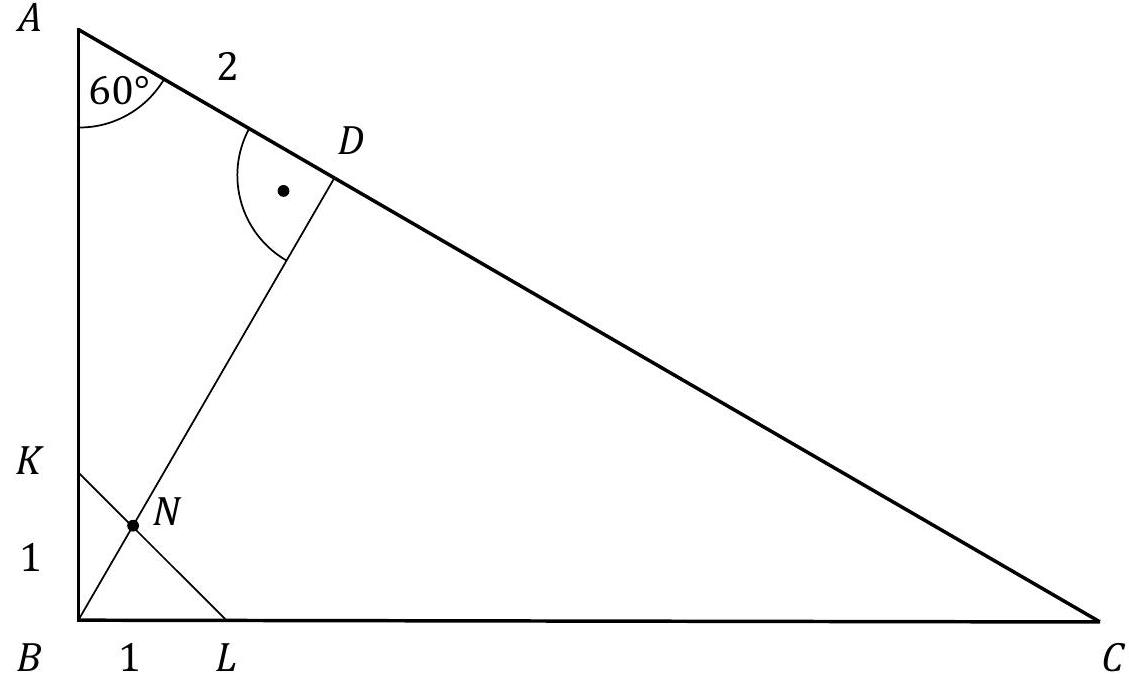
\includegraphics[max width=\textwidth, center]{2025_02_07_dcb3d059df06a3930b0ag-08}

W trójkącie $B L N$ miara kąta $N B L$ jest równa $60^{\circ}$. W trójkącie $K B N$ miara kąta $K B N$ jest równa $30^{\circ}$. Ponieważ pole trójkąta $K B L$ (równe $\frac{1}{2}$ ) jest sumą pól trójkątów $B L N$ oraz KBN, więc możemy zapisać równość

$$
\frac{1}{2} \cdot|B L| \cdot|B N| \cdot \sin 60^{\circ}+\frac{1}{2} \cdot|B N| \cdot|B K| \cdot \sin 30^{\circ}=\frac{1}{2}
$$

Stąd, po uwzględnieniu warunku $|B K|=|B L|=1$, otrzymujemy dalej

$$
\begin{gathered}
|B N| \cdot \frac{\sqrt{3}}{2}+|B N| \cdot \frac{1}{2}=1 \\
|B N| \cdot(\sqrt{3}+1)=2 \\
|B N|=\sqrt{3}-1
\end{gathered}
$$

Zatem $|N D|=|B D|-|B N|=2 \sqrt{3}-(\sqrt{3}-1)=\sqrt{3}+1$.\\
To należało wykazać.

\section*{Sposób II}
W trójkącie $D A B$ o kątach $90^{\circ}, 60^{\circ}, 30^{\circ}$ mamy: $|A D|=2,|A B|=4$ i $|B D|=2 \sqrt{3}$. Kąty w trójkącie $B N K$ mają miary: $30^{\circ}, 45^{\circ}, 105^{\circ}$. Stosujemy twierdzenie sinusów i zapisujemy równość:

$$
\frac{|B K|}{\sin 105^{\circ}}=\frac{|B N|}{\sin 45^{\circ}}
$$

Zatem

$$
|B N|=\frac{1 \cdot \sin 45^{\circ}}{\sin \left(60^{\circ}+45^{\circ}\right)}=\frac{\frac{\sqrt{2}}{2}}{\frac{\sqrt{3}}{2} \cdot \frac{\sqrt{2}}{2}+\frac{1}{2} \cdot \frac{\sqrt{2}}{2}}=\frac{2}{\sqrt{3}+1}=\sqrt{3}-1
$$

Ostatecznie $|N D|=|B D|-|B N|=2 \sqrt{3}-(\sqrt{3}-1)=\sqrt{3}+1$.\\
To należało wykazać.

\section*{Sposób III (trójkat BLN)}
Prowadzimy wysokość $N E$ w trójkącie $B L N$ i oznaczamy $x=|B E|$.\\
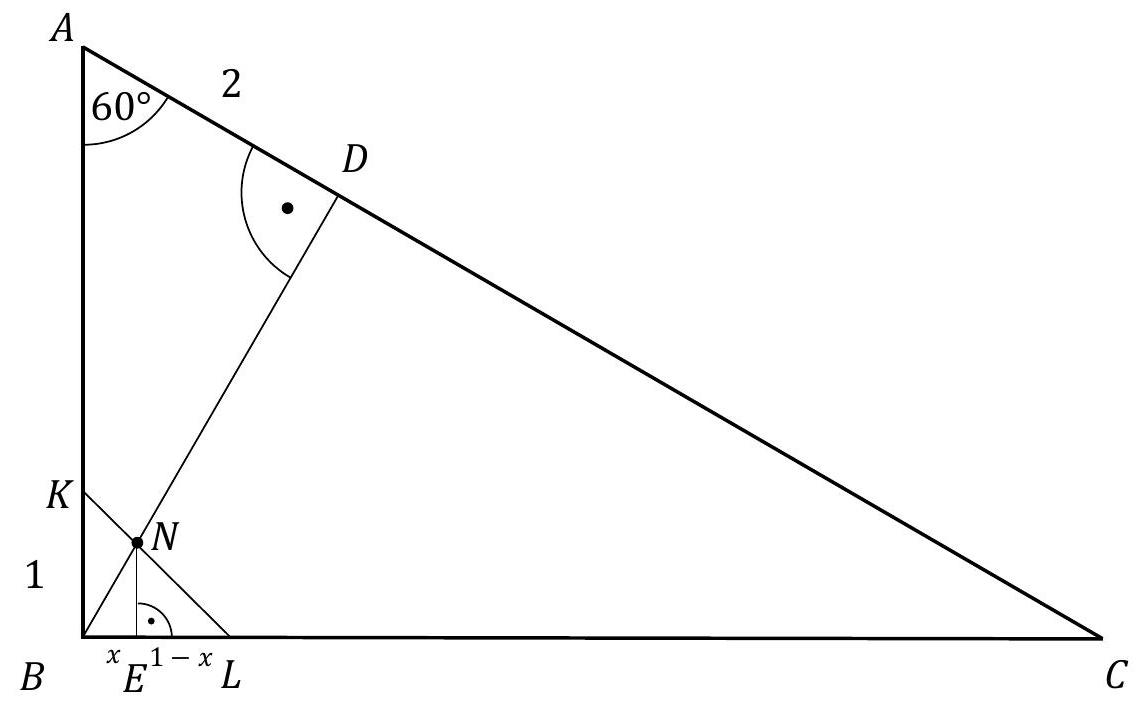
\includegraphics[max width=\textwidth, center]{2025_02_07_dcb3d059df06a3930b0ag-09}

Trójkąt prostokątny $D A B$ ma kąty ostre $60^{\circ}$ i $30^{\circ}$, więc:

$$
|A B|=2|A D|=2 \cdot 2=4 \quad \text { i } \quad|B D|=|A D| \sqrt{3}=2 \sqrt{3}
$$

Trójkąt prostokątny $B L K$ ma kąty ostre $45^{\circ}$, więc $|K L|=\sqrt{2}$.\\
W trójkącie prostokątnym NBE kąty ostre mają miary $60^{\circ}$ i $30^{\circ}$, więc

$$
|N E|=|B E| \cdot \sqrt{3}=x \sqrt{3} \quad \text { i }|B N|=2|B E|=2 x
$$

Trójkąt prostokątny $E L N$ ma kąty ostre $45^{\circ}$, więc

$$
|N E|=|E L|=x \sqrt{3}
$$

Ale $|N E|=|B L|-|B E|=1-x$, więc otrzymujemy równanie

$$
\begin{gathered}
1-x=x \sqrt{3} \\
x \sqrt{3}+x=1 \\
(\sqrt{3}+1) x=1
\end{gathered}
$$

Mnożąc obie strony równania przez $\sqrt{3}-1$, otrzymujemy

$$
2 x=\sqrt{3}-1
$$

czyli

$$
|B N|=2 x=\sqrt{3}-1
$$

Zatem $|N D|=|B D|-|B N|=2 \sqrt{3}-(\sqrt{3}-1)=\sqrt{3}+1$.\\
To należało wykazać.

\section*{Sposób IV (twierdzenie cosinusów)}
W trójkącie $D A B$ o kątach $90^{\circ}, 60^{\circ}, 30^{\circ}$ mamy: $|A D|=2,|A B|=4$ i $|B D|=2 \sqrt{3}$. W trójkącie $K B L$ kąty mają miary: $90^{\circ}, 45^{\circ}, 45^{\circ}$ oraz: $|B K|=|B L|=1,|K L|=\sqrt{2}$. Z twierdzenia cosinusów zastosowanego do trójkątów KBN oraz BLN otrzymujemy równości

$$
|B N|^{2}=|B K|^{2}+|K N|^{2}-2 \cdot|B K| \cdot|K N| \cdot \cos 45^{\circ}
$$

oraz

$$
|B N|^{2}=|B L|^{2}+|L N|^{2}-2 \cdot|B L| \cdot|L N| \cdot \cos 45^{\circ}
$$

Zatem po podstawieniu $|B K|=|B L|=1$ i dodaniu stronami równań otrzymujemy równość:

$$
2 \cdot|B N|^{2}=|L N|^{2}+|K N|^{2}
$$

Ponieważ $|\Varangle K B N|=30^{\circ}$, więc z twierdzenia cosinusów zastosowanego do trójkąta $K B N$ otrzymujemy:

$$
|K N|^{2}=|B K|^{2}+|B N|^{2}-2 \cdot|B K| \cdot|B N| \cdot \cos 30^{\circ}
$$

Ponieważ $|\Varangle N B L|=60^{\circ}$, więc z twierdzenia cosinusów zastosowanego do trójkąta BLN otrzymujemy:

$$
|L N|^{2}=|B L|^{2}+|B N|^{2}-2 \cdot|B L| \cdot|B N| \cdot \cos 60^{\circ}
$$

Zatem po podstawieniu $|B K|=|B L|=1$ i dodaniu stronami równań otrzymujemy równość:

$$
|L N|^{2}+|K N|^{2}=2+2 \cdot|B N|^{2}-|B N| \cdot \sqrt{3}-|B N|
$$

Ale

$$
2 \cdot|B N|^{2}=|L N|^{2}+|K N|^{2}
$$

więc

$$
2 \cdot|B N|^{2}=2+2 \cdot|B N|^{2}-|B N| \cdot \sqrt{3}-|B N|
$$

Zatem $|B N| \cdot(\sqrt{3}+1)=2$, czyli $|B N|=\sqrt{3}-1$. Dlatego\\
$|N D|=|B D|-|B N|=2 \sqrt{3}-(\sqrt{3}-1)=\sqrt{3}+1$.\\
To należało wykazać.

\section*{Sposób V (trójkat w układzie współrzędnych)}
Umieszczamy trójkąt $A B C$ w kartezjańskim układzie współrzędnych ( $x, y$ ) tak, aby: $B=(0,0), A$ był punktem leżącym na dodatniej półosi $O y, C$ był punktem leżącym na dodatniej półosi $O x$. Wtedy $K=(0,1)$ i $L=(1,0)$, więc prosta $K L$ ma równanie $y=-x+1$. Ponieważ $|\Varangle B A C|=60^{\circ}$ i $B D \perp A C$, więc prosta $B D$ jest nachylona do osi $O x$ pod kątem $60^{\circ}$. Stąd $B D$ ma równanie $y=\sqrt{3} x$.\\
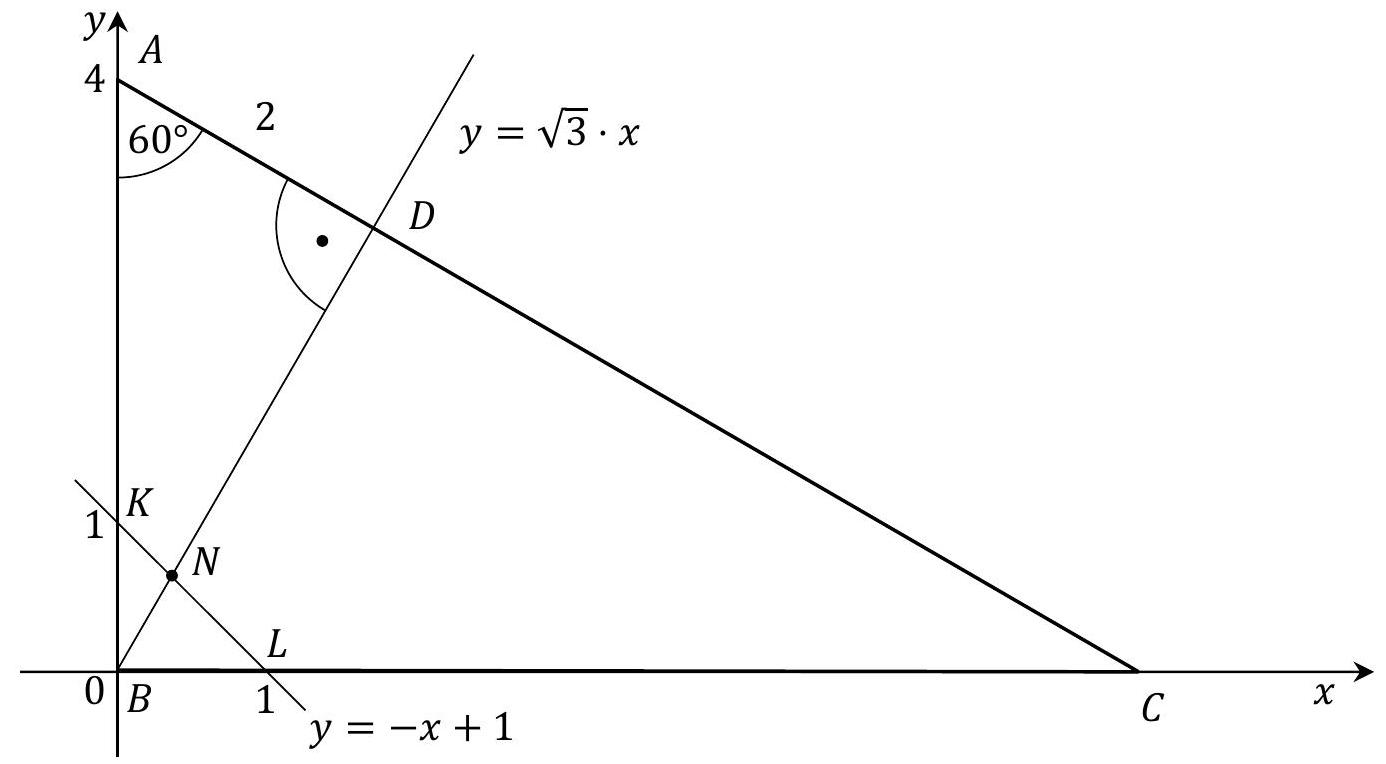
\includegraphics[max width=\textwidth, center]{2025_02_07_dcb3d059df06a3930b0ag-11}

Obliczamy współrzędne punktu $N$ :

$$
\begin{aligned}
& \left\{\begin{array}{l}
y=-x+1 \\
y=\sqrt{3} x
\end{array}\right. \\
& \left\{\begin{array}{l}
\sqrt{3} x=-x+1 \\
y=\sqrt{3} x
\end{array}\right. \\
& \left\{\begin{array}{l}
x=\frac{1}{\sqrt{3}+1} \\
y=\frac{\sqrt{3}}{\sqrt{3}+1}
\end{array}\right.
\end{aligned}
$$

czyli $N=\left(\frac{1}{\sqrt{3}+1}, \frac{\sqrt{3}}{\sqrt{3}+1}\right)$.\\
Obliczamy wspórzędne punktu $A$.\\
$\frac{|A D|}{|A B|}=\cos 60^{\circ}$, więc $|A B|=\frac{|A D|}{\cos 60^{\circ}}=4$ i stąd $A=(0,4)$.

Ponieważ $|\Varangle B C A|=30^{\circ}$, więc współczynnik kierunkowy a w równaniu prostej $A C$ jest równy $a=\operatorname{tg} 150^{\circ}=-\frac{\sqrt{3}}{3}$. Zatem prosta $A C$ ma równanie $y=-\frac{\sqrt{3}}{3} x+4$.\\
Obliczamy odległość punktu $N$ od prostej $A C$ :

$$
\begin{aligned}
& \frac{\left|-\frac{\sqrt{3}}{3} \cdot \frac{1}{\sqrt{3}+1}-1 \cdot \frac{\sqrt{3}}{\sqrt{3}+1}+4\right|}{\sqrt{\left(-\frac{\sqrt{3}}{3}\right)^{2}+(-1)^{2}}}=\frac{\left|\frac{-\sqrt{3}-3 \sqrt{3}+12(\sqrt{3}+1)}{3(\sqrt{3}+1)}\right|}{\frac{2}{\sqrt{3}}}=\frac{\frac{8 \sqrt{3}+12}{3(\sqrt{3}+1)}}{\frac{2}{\sqrt{3}}}= \\
& =\frac{8 \sqrt{3}+12}{3(\sqrt{3}+1) \cdot \frac{\sqrt{3}}{2}=\frac{4+2 \sqrt{3}}{\sqrt{3}+1}=\frac{2(2+\sqrt{3})(\sqrt{3}-1)}{2}=\sqrt{3}+1}
\end{aligned}
$$

Zatem $|N D|=\sqrt{3}+1$. To należało wykazać.\\
Sposób VI (prosta równoległa do KL przechodzaca przez D)\\
Prowadzimy wysokość $D E$ trójkąta $B C D$, a przez punkt $D$ prostą równoległą do prostej $K L$ i oznaczamy przez $F$ punkt jej przecięcia z prostą $B C$.\\
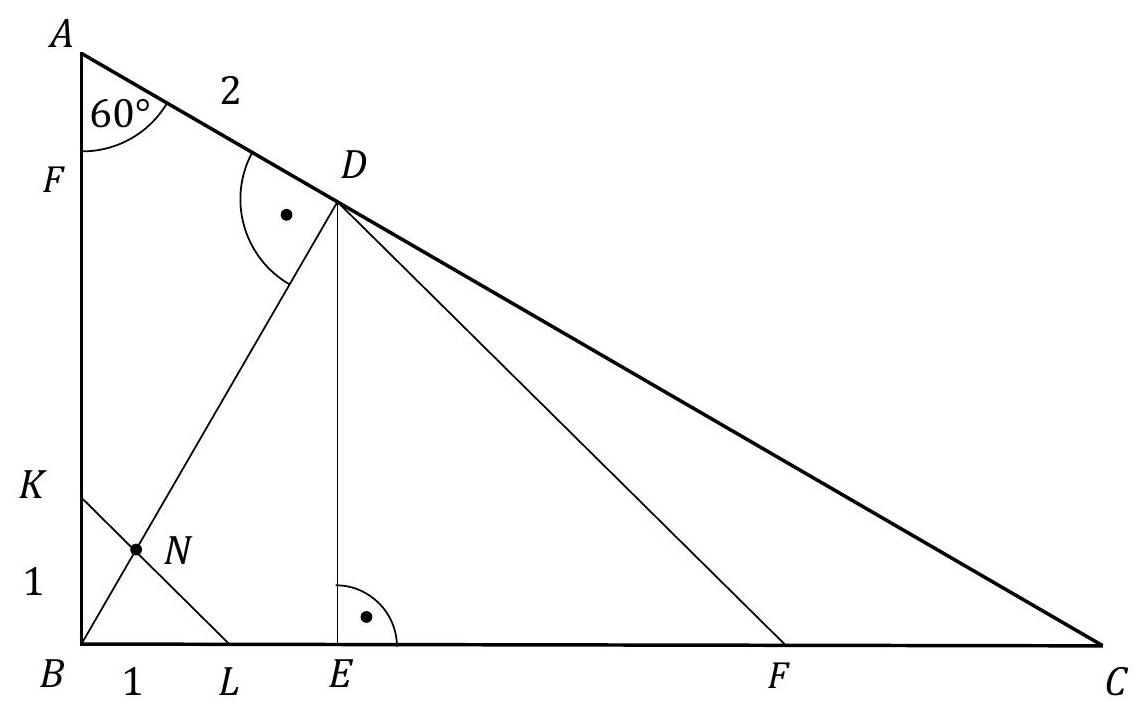
\includegraphics[max width=\textwidth, center]{2025_02_07_dcb3d059df06a3930b0ag-12}

W trójkącie $D A B$ o kątach $90^{\circ}, 60^{\circ}, 30^{\circ}$ mamy: $|A D|=2,|A B|=4$ i $|B D|=2 \sqrt{3}$.\\
Trójkąt prostokątny $B E D$ ma również kąty ostre $60^{\circ}$ i $30^{\circ}$, więc $|B E|=\frac{|B D|}{2}=\sqrt{3}$ i $|D E|=|B D| \sqrt{3}=3$.\\
Trójkąt prostokątny $D E F$ ma kąty ostre $45^{\circ}$, więc jest równoramienny.\\
Zatem $|E F|=|D E|=3$.\\
Stąd $|L F|=|L E|+|E F|=(|B E|-|B L|)+|E F|=\sqrt{3}-1+3=2+\sqrt{3}$.\\
Z twierdzenia Talesa otrzymujemy

$$
\frac{|N D|}{|L F|}=\frac{|B N|}{|B L|}
$$

czyli

$$
\frac{|N D|}{2+\sqrt{3}}=\frac{2 \sqrt{3}-|N D|}{1}
$$

Stąd

$$
\begin{gathered}
|N D|=(2+\sqrt{3}) \cdot(2 \sqrt{3}-|N D|) \\
|N D|+(2+\sqrt{3}) \cdot|N D|=4 \sqrt{3}+6 \\
|N D| \cdot(3+\sqrt{3})=4 \sqrt{3}+6 \\
|N D|=\frac{4 \sqrt{3}+6}{3+\sqrt{3}}=\frac{2(2 \sqrt{3}+3)(3-\sqrt{3})}{9-3}=\sqrt{3}+1
\end{gathered}
$$

To należało wykazać.

\section*{Sposób VII (prosta równoległa do BC przechodzaca przez D)}
Prowadzimy przez punkt $D$ prostą równoległą do prostej $B C$ i oznaczamy przez $E$ punkt jej przecięcia z prostą $K L$, natomiast przez $F$ - punkt jej przecięcia z prostą $A B$.\\
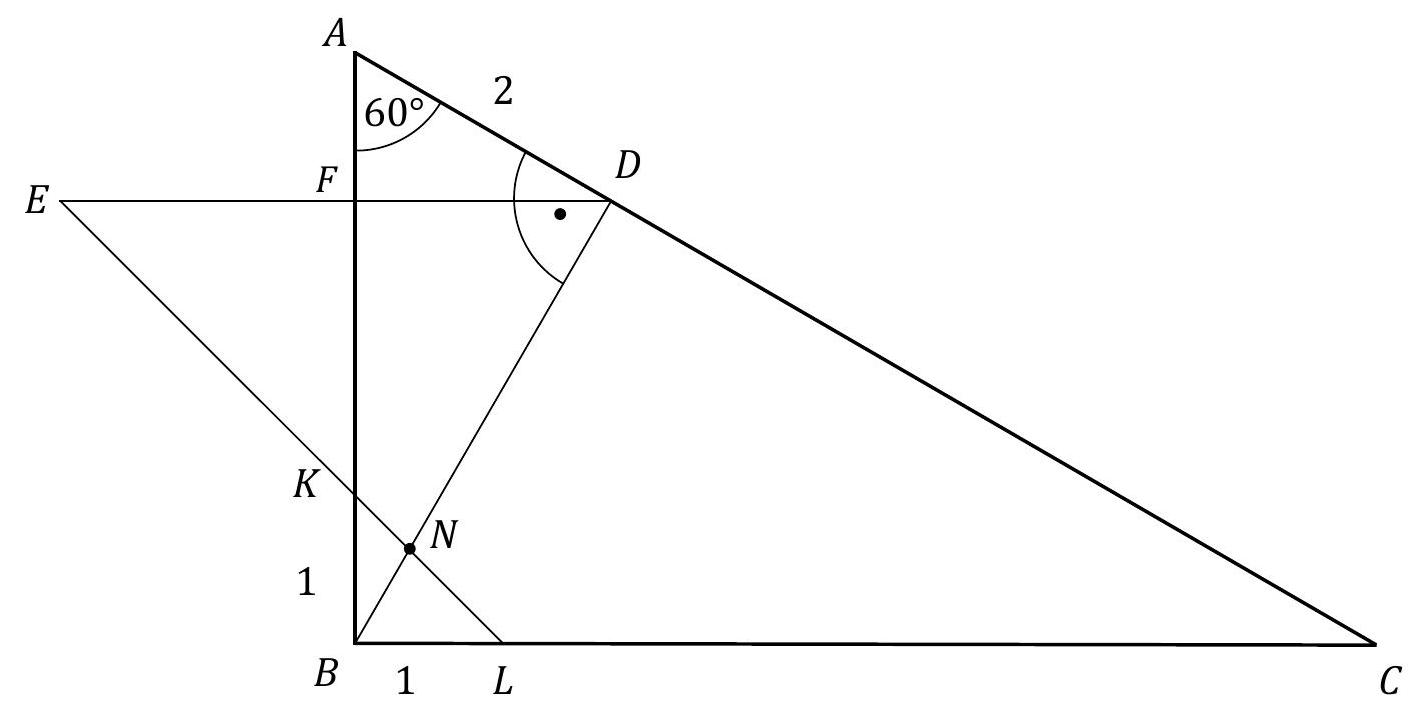
\includegraphics[max width=\textwidth, center]{2025_02_07_dcb3d059df06a3930b0ag-13}

W trójkącie $D A B$ o kątach $90^{\circ}, 60^{\circ}, 30^{\circ}$ mamy: $|A D|=2,|A B|=4$ i $|B D|=2 \sqrt{3}$.\\
Trójkąt prostokątny $A F D$ ma kąty ostre $60^{\circ}$ i $30^{\circ}$, więc $|A F|=1$ oraz $|D F|=\sqrt{3}$.\\
Zatem $|F K|=4-1-1=2$.\\
Trójkąt prostokątny $K F E$ ma kąty ostre $45^{\circ}$, więc jest równoramienny.\\
Zatem $|E F|=|F K|=2$. Stąd $|E D|=2+\sqrt{3}$.\\
Trójkąty $D E N$ i $B L N$ są podobne ( $k k k$ ), więc

$$
\frac{|N D|}{|E D|}=\frac{|B N|}{|B L|}
$$

czyli

Egzamin maturalny z matematyki na poziomie rozszerzonym - termin główny 2023 r.

$$
\frac{|N D|}{2+\sqrt{3}}=\frac{2 \sqrt{3}-|N D|}{1}
$$

Stąd

$$
\begin{gathered}
|N D|=(2+\sqrt{3}) \cdot(2 \sqrt{3}-|N D|) \\
|N D|+(2+\sqrt{3}) \cdot|N D|=4 \sqrt{3}+6 \\
|N D| \cdot(3+\sqrt{3})=4 \sqrt{3}+6 \\
|N D|=\frac{4 \sqrt{3}+6}{3+\sqrt{3}}=\frac{2(2 \sqrt{3}+3)(3-\sqrt{3})}{9-3}=\sqrt{3}+1
\end{gathered}
$$

To należało wykazać.

Zadanie 8. (0-3)

\begin{center}
\begin{tabular}{|l|l|}
\hline
\multicolumn{2}{|c|}{Wymagania egzaminacyjne 2023 i 2024} \\
\hline
\multicolumn{1}{|c|}{Wymaganie ogólne} & \multicolumn{1}{|c|}{Wymaganie szczegółowe} \\
\hline
III. Modelowanie matematyczne. & Zdający: \\
 & R10.3) korzysta z twierdzenia \\
 & o prawdopodobieństwie całkowitym. \\
\hline
\end{tabular}
\end{center}

\section*{Zasady oceniania}
3 pkt - zastosowanie poprawnej metody obliczenia prawdopodobieństwa i poprawny wynik: $\frac{2}{7}$.\\
2 pkt - zapisanie/obliczenie prawdopodobieństwa zdarzeń $B_{1}, B_{2}, B_{3}$ oraz prawdopodobieństw warunkowych $P\left(A \mid B_{1}\right), P\left(A \mid B_{2}\right), P\left(A \mid B_{3}\right)$ :

$$
P\left(B_{1}\right)=\frac{\binom{5}{2}}{\binom{7}{2}} \text { i } P\left(B_{2}\right)=\frac{\binom{5}{1} \cdot\binom{2}{1}}{\binom{7}{2}} \text {, } P\left(B_{3}\right)=\frac{\binom{2}{2}}{\binom{7}{2}} \text {, } P\left(A \mid B_{1}\right)=\frac{2}{5} \text {, i } P\left(A \mid B_{2}\right)=\frac{1}{5} \text {, }
$$

$$
\text { i } P\left(A \mid B_{3}\right)=0
$$

ALBO

\begin{itemize}
  \item zapisanie prawdopodobieństw na wszystkich odcinkach istotnych gałęzi drzewa, ALBO
  \item zapisanie/obliczenie liczby wszystkich zdarzeń elementarnych oraz liczby wszystkich zdarzeń elementarnych sprzyjających zdarzeniu $A$, przy zastosowaniu klasycznej definicji prawdopodobieństwa: $|\Omega|=7 \cdot 6 \cdot 5$ oraz
\end{itemize}

$$
\left.|A|=5 \cdot 4 \cdot 2+5 \cdot 2 \cdot 1+2 \cdot 5 \cdot 1 \quad \text { (lub }|A|=\left|A_{1}\right|+\left|A_{2}\right|+\left|A_{3}\right|=60\right) .
$$

1 pkt - opisanie zdarzeń losowych $B_{1}, B_{2}, B_{3}$ i obliczenie ich prawdopodobieństw:\\
$P\left(B_{1}\right)=\frac{\binom{5}{2}}{\binom{7}{2}}, P\left(B_{2}\right)=\frac{\binom{5}{1} \cdot\binom{2}{1}}{\binom{7}{2}}, P\left(B_{3}\right)=\frac{\binom{2}{2}}{\binom{7}{2}}$\\
ALBO

\begin{itemize}
  \item narysowanie drzewa stochastycznego doświadczenia i zapisanie prawdopodobieństw na gałęziach drzewa I etapu doświadczenia (dla drzewa dwuetapowego) lub I i II etapu (dla drzewa trzyetapowego),\\
ALBO
  \item obliczenie prawdopodobieństw wylosowania kuli czarnej na ostatnim etapie oraz właściwe zinterpretowanie wcześniejszych etapów doświadczenia: $\frac{2}{5}, \frac{1}{5}$,\\
ALBO
  \item zapisanie/obliczenie liczby wszystkich zdarzeń elementarnych lub liczby wszystkich zdarzeń elementarnych sprzyjających zdarzeniu $A$, przy zastosowaniu klasycznej definicji prawdopodobieństwa: $|\Omega|=7 \cdot 6 \cdot 5$ lub\\
$|A|=5 \cdot 4 \cdot 2+5 \cdot 2 \cdot 1+2 \cdot 5 \cdot 1$ (lub $|A|=\left|A_{1}\right|+\left|A_{2}\right|+\left|A_{3}\right|=60$ ).\\
0 pkt - rozwiązanie, w którym zastosowano nieprawidłową metodę, albo brak rozwiązania.
\end{itemize}

\section*{Uwagi:}
\begin{enumerate}
  \item Jeżeli zdający, stosując twierdzenie o prawdopodobieństwie całkowitym, pominie składnik $P\left(B_{3}\right) \cdot P\left(A \mid B_{3}\right)$, to może otrzymać $\mathbf{3}$ punkty za całe rozwiązanie
  \item Jeżeli zdający zapisze jedynie $P(A)=\frac{2}{7}$, to otrzymuje 1 punkt.
  \item Jeżeli zdający zapisze $P(A)=\frac{2}{7}$ i zapisze poprawny komentarz uzasadniający otrzymany wynik, to otrzymuje 3 punkty.
\end{enumerate}

\section*{Przykładowe pełne rozwiązania}
Sposób I (prawdopodobieństwo całkowite)\\
Wprowadzamy następujące oznaczenia:\\
$A$ - zdarzenie polegające na tym, że w drugim losowaniu wylosowano kulę czarną,\\
$B_{1}$ - zdarzenie polegające na tym, że w pierwszym losowaniu wylosowano dwie kule białe, $B_{2}$ - zdarzenie polegające na tym, że w pierwszym losowaniu wylosowano kulę białą i kulę czarna,\\
$B_{3}$ - zdarzenie polegające na tym, że w pierwszym losowaniu wylosowano dwie kule czarne.\\
Obliczamy prawdopodobieństwa zdarzeń $B_{1}, B_{2}, B_{3}$ :

$$
P\left(B_{1}\right)=\frac{\binom{5}{2}}{\binom{7}{2}}=\frac{10}{21} \quad P\left(B_{2}\right)=\frac{\binom{5}{1} \cdot\binom{2}{1}}{\binom{7}{2}}=\frac{10}{21} \quad P\left(B_{3}\right)=\frac{\binom{2}{2}}{\binom{7}{2}}=\frac{1}{21}
$$

Obliczamy prawdopodobieństwa warunkowe $P\left(A \mid B_{1}\right), P\left(A \mid B_{2}\right), P\left(A \mid B_{3}\right)$ :

$$
\begin{gathered}
P\left(A \mid B_{1}\right)=P\left(A \cap B_{1}\right): P\left(B_{1}\right)=\frac{\binom{5}{2} \cdot\binom{2}{1}}{\binom{7}{2} \cdot\binom{5}{1}}: \frac{\binom{5}{2}}{\binom{7}{2}}=\frac{2}{5} \\
P\left(A \mid B_{2}\right)=\frac{1}{5} \quad P\left(A \mid B_{3}\right)=0
\end{gathered}
$$

Stosujemy twierdzenie o prawdopodobieństwie całkowitym i obliczamy prawdopodobieństwo zdarzenia $A$ :

$$
\begin{aligned}
P(A) & =P\left(A \mid B_{1}\right) \cdot P\left(B_{1}\right)+P\left(A \mid B_{2}\right) \cdot P\left(B_{2}\right)+P\left(A \mid B_{3}\right) \cdot P\left(B_{3}\right)= \\
& =\frac{2}{5} \cdot \frac{10}{21}+\frac{1}{5} \cdot \frac{10}{21}+0 \cdot \frac{1}{21}=\frac{2}{7}
\end{aligned}
$$

\section*{Sposób II (model klasyczny)}
Niech $K$ będzie zbiorem siedmiu kul, które znajdowały się w pojemniku. Przyjmijmy, że zdarzeniem elementarnym jest każdy ciąg ( $x, y, z$ ), którego wyrazami są trzy kule: $x, y, z \in K$, parami różne. Zdarzenia elementarne są jednakowo prawdopodobne (jest to model klasyczny).\\
Wtedy

$$
|\Omega|=7 \cdot 6 \cdot 5=210
$$

gdzie $|\Omega|$ oznacza liczbę elementów zbioru $\Omega$ (zbioru wszystkich zdarzeń elementarnych).

Niech $A$ będzie zdarzeniem polegającym na tym, że trzecia z wylosowanych kul (z) będzie czarna.\\
Zdarzenie $A$ jest sumą parami rozłącznych zdarzeń:\\
$A_{1}$ - dwie wylosowane kule ( $x$ oraz $y$ ) będą białe, a trzecia kula ( $z$ ) będzie czarna,\\
$A_{2}$ - pierwsza kula ( $x$ ) będzie biała, a następne dwie ( $y$ oraz $z$ ) będą czarne,\\
$A_{3}$ - pierwsza kula ( $x$ ) będzie czarna, druga $(y)$ będzie biała, a trzecia kula ( $z$ ) będzie czarna.\\
Ponieważ

$$
\left|A_{1}\right|=5 \cdot 4 \cdot 2=40, \quad\left|A_{2}\right|=5 \cdot 2 \cdot 1=10, \quad\left|A_{3}\right|=2 \cdot 5 \cdot 1=10
$$

więc

$$
|A|=\left|A_{1}\right|+\left|A_{2}\right|+\left|A_{3}\right|=60
$$

Prawdopodobieństwo zdarzenia $A$ jest równe

$$
P(A)=\frac{|A|}{|\Omega|}=\frac{60}{210}=\frac{2}{7}
$$

\section*{Sposób III (drzewo stochastyczne - 3 etapy)}
Rysujemy fragment drzewa stochastycznego rozważanego doświadczenia z uwzględnieniem wszystkich istotnych gałęzi. Symbol „b" odpowiada wylosowaniu kuli białej, symbol „c" - kuli czarnej. Po wylosowaniu dwóch kul czarnych nie możemy już wylosować kuli czarnej.\\
Oznaczamy przez $A$ zdarzenie polegające na tym, że trzecia z wylosowanych kul jest czarna.\\
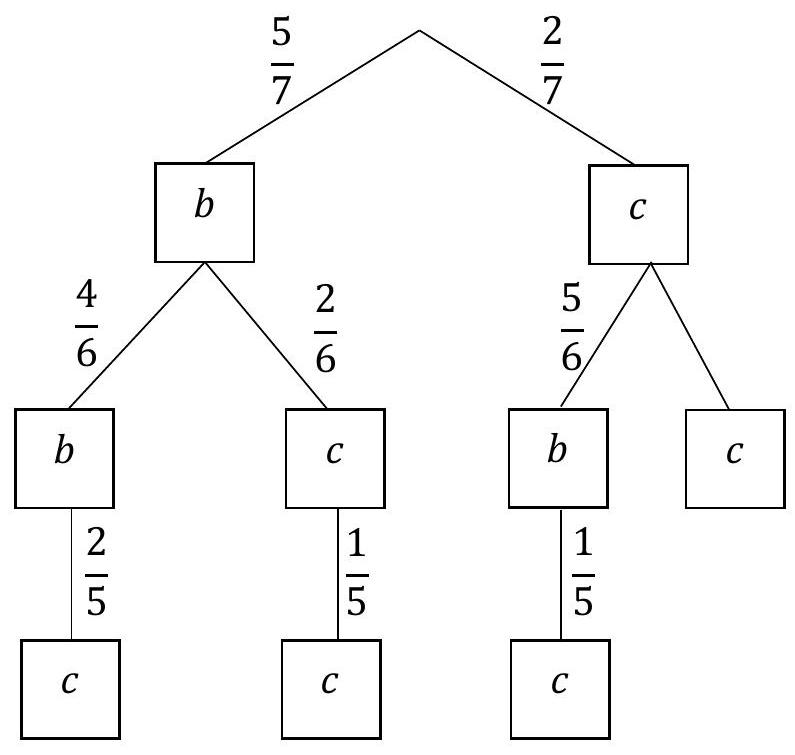
\includegraphics[max width=\textwidth, center]{2025_02_07_dcb3d059df06a3930b0ag-17}

Prawdopodobieństwo zdarzenia $A$ jest równe

$$
P(A)=\frac{5}{7} \cdot \frac{4}{6} \cdot \frac{2}{5}+\frac{5}{7} \cdot \frac{2}{6} \cdot \frac{1}{5}+\frac{2}{7} \cdot \frac{5}{6} \cdot \frac{1}{5}=\frac{2}{7}
$$

\section*{Sposób III (drzewo stochastyczne - 2 etapy)}
Rysujemy fragment drzewa stochastycznego rozważanego doświadczenia z uwzględnieniem wszystkich istotnych gałęzi. Symbol „b" odpowiada kuli białej, symbol „c" - kuli czarnej.\\
Po wylosowaniu dwóch kul czarnych nie możemy już wylosować kuli czarnej.\\
Oznaczamy przez A zdarzenie polegające na tym, że kula wylosowana w drugim losowaniu jest czarna.\\
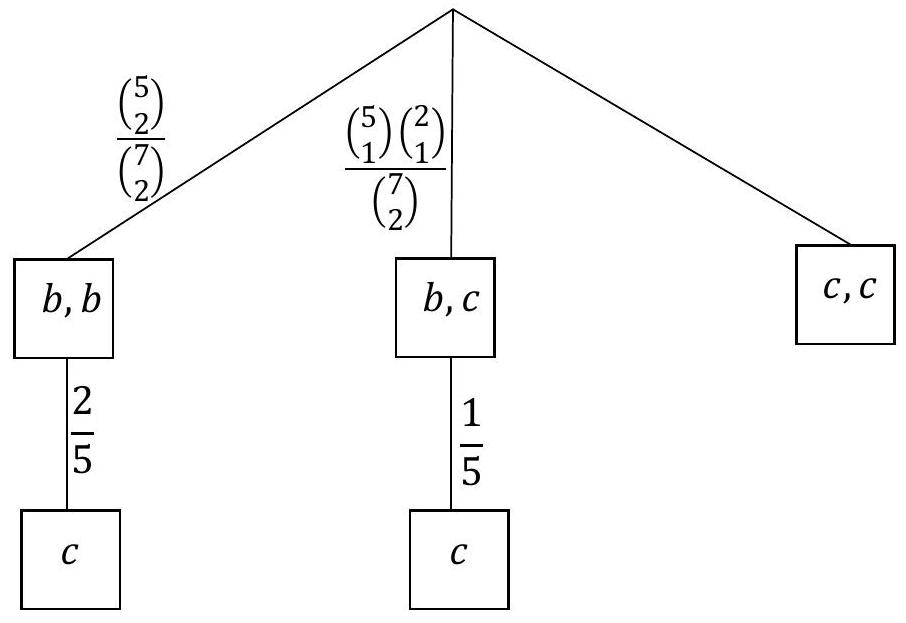
\includegraphics[max width=\textwidth, center]{2025_02_07_dcb3d059df06a3930b0ag-18}

Prawdopodobieństwo zdarzenia $A$ jest równe

$$
P(A)=\frac{\binom{5}{2}}{\binom{7}{2}} \cdot \frac{2}{5}+\frac{\binom{5}{2}}{\binom{7}{2}} \cdot \frac{1}{5}=\frac{2}{7}
$$

\section*{Zadanie 9. (0-3)}
\begin{center}
\begin{tabular}{|l|l|}
\hline
\multicolumn{2}{|c|}{Wymagania egzaminacyjne 2023 i 2024} \\
\hline
\multicolumn{1}{|c|}{Wymaganie ogólne} & \multicolumn{1}{|c|}{Wymagania szczegółowe} \\
\hline
V. Rozumowanie i argumentacja. & Zdajacy: \\
 & R11.2) oblicza pochodne funkcji \\
 & wymiernych; \\
 & R11.3) korzysta z geometrycznej \\
 & interpretacji pochodnej. \\
\hline
\end{tabular}
\end{center}

\section*{Zasady oceniania}
3 pkt - zastosowanie poprawnej metody i poprawny wynik: $x_{0}=-3$ oraz $y=-\frac{8}{11} x+\frac{9}{11}$ (lub $\left.y=-\frac{8}{11}(x+3)+3\right)$.\\
2 pkt - obliczenie odciętej punktu $P$ i wyznaczenie pochodnej funkcji $f: x_{0}=-3$ oraz

$$
f^{\prime}(x)=\frac{(6 x-2) \cdot\left(x^{2}+2 x+8\right)-\left(3 x^{2}-2 x\right) \cdot(2 x+2)}{\left(x^{2}+2 x+8\right)^{2}} .
$$

1 pkt - obliczenie odciętej punktu $P: x_{0}=-3$\\
ALBO

\begin{itemize}
  \item wyznaczenie pochodnej funkcji $f: f^{\prime}(x)=\frac{(6 x-2) \cdot\left(x^{2}+2 x+8\right)-\left(3 x^{2}-2 x\right) \cdot(2 x+2)}{\left(x^{2}+2 x+8\right)^{2}}$.
\end{itemize}

0 pkt - rozwiązanie, w którym zastosowano niepoprawną metodę, albo brak rozwiązania.

\section*{Uwaga:}
Jeżeli zdający błędnie stosuje wzór na pochodną ilorazu funkcji, to może otrzymać co najwyżej 1 punkt za całe rozwiązanie.

\section*{Przykładowe pełne rozwiązanie}
Obliczamy odciętą $x_{0}$ punktu $P$ :

$$
\begin{gathered}
3=\frac{3 x_{0}^{2}-2 x_{0}}{x_{0}^{2}+2 x_{0}+8} \\
3 x_{0}^{2}+6 x_{0}+24=3 x_{0}^{2}-2 x_{0} \\
x_{0}=-3
\end{gathered}
$$

Wyznaczamy pochodną funkcji $f$ :

$$
\begin{gathered}
f^{\prime}(x)=\frac{(6 x-2)\left(x^{2}+2 x+8\right)-\left(3 x^{2}-2 x\right)(2 x+2)}{\left(x^{2}+2 x+8\right)^{2}} \\
f^{\prime}(x)=\frac{8 x^{2}+48 x-16}{\left(x^{2}+2 x+8\right)^{2}}
\end{gathered}
$$

Wyznaczamy równanie kierunkowe $y=a x+b$ stycznej do wykresu funkcji $f$ w punkcie $P$. Obliczamy współczynnik kierunkowy $a$ w równaniu stycznej:

$$
a=f^{\prime}(-3)=-\frac{8}{11}
$$

Obliczamy współczynnik b w równaniu stycznej:

$$
\begin{gathered}
3=-\frac{8}{11} \cdot(-3)+b \\
b=\frac{9}{11}
\end{gathered}
$$

Styczna ma równanie $y=-\frac{8}{11} x+\frac{9}{11}$.

Zadanie 10. (0-4)

\begin{center}
\begin{tabular}{|l|l|}
\hline
\multicolumn{1}{|c|}{Wymagania egzaminacyjne 2023 i 2024} &  \\
\hline
\multicolumn{1}{|c|}{Wymaganie ogólne} & \multicolumn{1}{c|}{Wymaganie szczegółowe} \\
\hline
II. Wykorzystanie i interpretowanie & Zdający: \\
reprezentacji. & R3.8) rozwiązuje równania i nierówności \\
 & z wartością bezwzględna, o poziomie \\
 & trudności nie wyższym niż: \\
 & $||x+1|-2|=3,|x+3|+|x-5|>12$. \\
\hline
\end{tabular}
\end{center}

\section*{Zasady oceniania}
4 pkt - zastosowanie poprawnej metody i poprawny wynik: $x \in\left(-\frac{11}{3}, \frac{14}{3}\right)$.\\
3 pkt - rozwiązanie nierówności w dwóch spośród rozważanych przedziałów/przypadków (o ile rozpatruje nierówność w przedziałach/przypadkach, których suma jest równa $\mathbb{R} /$ wyczerpujących zbiór $\mathbb{R}$ )

\section*{ALBO}
\begin{itemize}
  \item zapisanie nierówności w postaci równoważnej koniunkcji dwóch nierówności:\\
$x+2<\frac{25}{3}-|x-3|$ i $x+2>-\left(\frac{25}{3}-|x-3|\right)$, a następnie w postaci równoważnej koniunkcji nierówności bez użycia symbolu wartości bezwzględnej:\\
$x-3<\frac{19}{3}-x$ i $x-3>-\left(\frac{19}{3}-x\right)$ i $x-3<x+\frac{31}{3}$ i $x-3>-\left(x+\frac{31}{3}\right)$, ALBO
  \item odczytanie z wykresów funkcji $f$ oraz $g$ pierwszych współrzędnych punktów ich przecięcia: $x=-\frac{11}{3}$ oraz $x=\frac{14}{3}$ i sprawdzenie rachunkiem poprawności odczytanych współrzędnych.\\
2 pkt - zastosowanie definicji wartości bezwzględnej lub własności wartości bezwzględnej i zapisanie danej nierówności odpowiednio w trzech przedziałach: $(-\infty,-2)$, $\langle-2,3),(3,+\infty)$, lub w czterech przypadkach: $x+2<0$ i $x-3<0, x+2<0$ i $x-3 \geq 0, x+2 \geq 0$ i $x-3<0, x+2 \geq 0$ i $x-3 \geq 0$ (z dokładnością do domknięcia)\\
ALBO
  \item zapisanie nierówności w postaci równoważnej koniunkcji dwóch nierówności:\\
$x+2<\frac{25}{3}-|x-3|$ i $x+2>-\left(\frac{25}{3}-|x-3|\right)$,\\
ALBO
  \item narysowanie wykresów funkcji $f(x)=|x+2|$ oraz $g(x)=\frac{25}{3}-|x-3|$.
\end{itemize}

1 pkt - przekształcenie danej nierówności do postaci $|x+2|<\frac{25}{3}-|x-3|$.\\
0 pkt - rozwiązanie, w którym zastosowano niepoprawną metodę, albo brak rozwiązania.

\section*{Uwagi:}
\begin{enumerate}
  \item Jeśli w rozwiązaniu algebraicznym zdający popełni błąd przy zapisie nierówności tylko w jednym z rozpatrywanych przypadków, ale konsekwentnie do popełnionego błędu rozwiąże zadanie do końca, to może uzyskać co najwyżej 2 punkty za całe rozwiązanie.
  \item Jeśli w rozwiązaniu graficznym zdający popełni jeden błąd przy rysowaniu wykresu funkcji $f(x)=|x+2|$ albo $g(x)=\frac{25}{3}-|x-3|$, ale otrzyma dwa punkty przecięcia i dalej konsekwentnie do popełnionego błędu rozwiąże zadanie do końca, to może uzyskać co najwyżej 2 punkty za całe rozwiązanie (za zapisanie wyrażeń w postaci $|x+2|$ oraz $|x-3|$ oraz konsekwentną interpretację zbioru rozwiązań).
  \item Jeżeli zdający przy rozwiązaniu graficznym poda zbiór rozwiązań $x \in\left(-\frac{11}{3}, \frac{14}{3}\right)$, ale nie sprawdzi rachunkiem pierwszych współrzędnych punktów przecięcia wykresów funkcji $f$ i $g$, to może otrzymać co najwyżej 3 punkty za całe rozwiązanie.
\end{enumerate}

\section*{Przykładowe pełne rozwiązania}
Sposób 1\\
Zauważamy, że $\sqrt{x^{2}+4 x+4}=\sqrt{(x+2)^{2}}=|x+2|$ oraz\\
$\sqrt{x^{2}-6 x+9}=\sqrt{(x-3)^{2}}=|x-3|$.\\
Zapisujemy nierówność $\sqrt{x^{2}+4 x+4}<\frac{25}{3}-\sqrt{x^{2}-6 x+9}$ w równoważnej postaci $|x+2|<\frac{25}{3}-|x-3|$.\\
Rozważamy trzy przypadki.\\
Przypadek 1. (gdy $x \in(-\infty,-2))$\\
W tym przypadku nierówność ma postać $-x-2<\frac{25}{3}+x-3$, czyli $x>-\frac{11}{3}$.\\
Stąd otrzymujemy $x \in\left(-\frac{11}{3},-2\right)$.\\
Przypadek 2. (gdy $x \in\langle-2,3)$ )\\
W tym przypadku nierówność ma postać $x+2<\frac{25}{3}+x-3$. Otrzymujemy prawdziwą nierówność $5<\frac{25}{3}$, więc $x \in\langle-2,3)$.

Przypadek 3. (gdy $x \in\langle 3,+\infty)$ )\\
W tym przypadku nierówność ma postać $x+2<\frac{25}{3}-x+3$, czyli $x<\frac{14}{3}$. Stąd otrzymujemy $x \in\left(3, \frac{14}{3}\right)$.\\
Ostatecznie rozwiązaniami danej nierówności są wszystkie liczby ze zbioru $\left(-\frac{11}{3}, \frac{14}{3}\right)$.

\section*{Sposób II (poprzez koniunkcję nierówności)}
Zauważamy, że $\sqrt{x^{2}+4 x+4}=\sqrt{(x+2)^{2}}=|x+2|$ oraz $\sqrt{x^{2}-6 x+9}=\sqrt{(x-3)^{2}}=|x-3|$.\\
Zapisujemy nierówność $\sqrt{x^{2}+4 x+4}<\frac{25}{3}-\sqrt{x^{2}-6 x+9}$ w równoważnej postaci $|x+2|<\frac{25}{3}-|x-3|$.\\
Dla każdej liczby rzeczywistej $x$ i dla każdej liczby rzeczywistej $a$ prawdziwa jest równoważność: $|x|<a$ wtedy i tylko wtedy, gdy $x<a$ i $x>-a$.

Przekształcamy nierówność $|x+2|<\frac{25}{3}-|x-3|$, korzystając z tej równoważności dwukrotnie:

$$
\begin{gathered}
x+2<\frac{25}{3}-|x-3| \quad \text { i } x+2>-\left(\frac{25}{3}-|x-3|\right) \\
|x-3|<\frac{19}{3}-x \quad \text { i }|x-3|<x+\frac{31}{3} \\
x-3<\frac{19}{3}-x \text { i } x-3>-\left(\frac{19}{3}-x\right) \quad \text { i } x-3<x+\frac{31}{3} \quad \text { i } x-3>-\left(x+\frac{31}{3}\right) \\
2 x<\frac{28}{3} \text { i }-3>-\frac{19}{3} \text { i }-3<\frac{31}{3} \text { i } 2 x>-\frac{22}{3} \\
x<\frac{14}{3} \quad \text { i } x \in \mathbb{R} \quad \text { i } x \in \mathbb{R} \quad \text { i } x>-\frac{11}{3} \\
-\frac{11}{3}<x<\frac{14}{3}
\end{gathered}
$$

Ostatecznie rozwiązaniami danej nierówności są wszystkie liczby ze zbioru $\left(-\frac{11}{3}, \frac{14}{3}\right)$.

Zadanie 11. (0-4)

\begin{center}
\begin{tabular}{|l|l|}
\hline
\multicolumn{2}{|c|}{Wymagania egzaminacyjne 2023 i 2024} \\
\hline
\multicolumn{1}{|c|}{Wymaganie ogólne} & \multicolumn{1}{c|}{Wymaganie szczegółowe} \\
\hline
III. Modelowanie matematyczne. & Zdajacy: \\
 & R5.2) rozpoznaje szeregi geometryczne \\
 & zbieżne i oblicza ich sumy. \\
\hline
\end{tabular}
\end{center}

\section*{Zasady oceniania}
4 pkt - zastosowanie poprawnej metody i poprawny wynik: $L=\frac{4 a}{1-\frac{\sqrt{10}}{4}}$ (lub $L=\frac{8 \cdot(4+\sqrt{10}) a}{3}$ ).\\
3 pkt - zapisanie: $L=4 a\left(1+\frac{\sqrt{10}}{4}+\frac{5}{8}+\ldots\right)$.\\
2 pkt - obliczenie ilorazu ciągu: $q=\frac{\sqrt{10}}{4}$.\\
1 pkt - obliczenie długości boku drugiego kwadratu: $a_{2}=\frac{\sqrt{10}}{4} a$.\\
0 pkt - rozwiązanie, w którym zastosowano niepoprawną metodę, albo brak rozwiązania.

\section*{Uwagi:}
\begin{enumerate}
  \item Jeżeli zdający obliczy tylko sumę długości boków (po jednym z każdego kwadratu), to może otrzymać co najwyżej 3 punkty za całe rozwiązanie.
  \item Jeżeli zdający błędnie ustala stosunek podziału długości boku kwadratu i rozwiązuje zadanie konsekwentnie do końca, to może otrzymać co najwyżej 2 punkty za całe rozwiązanie (za obliczenie ilorazu $q$ ciągu, o ile $q \in(0,1)$, oraz za konsekwentne obliczenie sumy obwodów wszystkich kwadratów).
  \item Jeżeli zdający przyjmuje do obliczeń konkretną długość boku kwadratu $K_{1}$ i rozwiązuje zadanie konsekwentnie do końca, to otrzymuje 2 punkty za całe rozwiązanie.
  \item Jeżeli zdający popełni błąd rachunkowy i otrzyma iloraz $q$ ciągu, który jest liczbą spoza przedziału ( 0,1 ), to może otrzymać co najwyżej 1 punkt za całe rozwiązanie (za poprawne obliczenie $a_{2}$ ).
\end{enumerate}

\section*{Przykładowe pełne rozwiązanie}
Oznaczmy przez $a_{i}$ długość boku kwadratu $K_{i}$, natomiast przez $L_{i}$ - obwód kwadratu $K_{i}$ (dla $i=1,2,3, \ldots$ ). Niech $L$ oznacza sumę obwodów wszystkich rozważanych kwadratów. Obliczamy długości boków kolejnych kwadratów:

$$
\begin{gathered}
a_{1}=a \\
a_{2}=\sqrt{\left(\frac{1}{4} a\right)^{2}+\left(\frac{3}{4} a\right)^{2}}=\frac{\sqrt{10}}{4} a
\end{gathered}
$$

Analogicznie

$$
\begin{gathered}
a_{3}=\frac{\sqrt{10}}{4} a_{2}=\frac{\sqrt{10}}{4} \cdot \frac{\sqrt{10}}{4} a=\frac{5}{8} a \\
a_{4}=\frac{5 \sqrt{10}}{32} a
\end{gathered}
$$

i tak dalej.\\
Stąd

$$
L=L_{1}+L_{2}+L_{3}+\ldots=4 a+4 \cdot \frac{\sqrt{10}}{4} a+4 \cdot \frac{5}{8} a+\ldots=4 a\left(1+\frac{\sqrt{10}}{4}+\frac{5}{8}+\ldots\right)
$$

Zauważamy, że wyrażenie w nawiasie jest sumą szeregu geometrycznego, gdzie $a_{1}=1$\\
i $q=\frac{\sqrt{10}}{4}$.\\
Ponieważ $|q|=\frac{\sqrt{10}}{4}<1$, zatem spełnione są założenia twierdzenia o istnieniu sumy nieskończonego szeregu geometrycznego.\\
Zatem $L=4 a \cdot \frac{1}{1-\frac{\sqrt{10}}{4}}=\frac{4 a}{1-\frac{\sqrt{10}}{4}}=\frac{8 \cdot(4+\sqrt{10}) a}{3}$.

\section*{Zadanie 12. (0-4)}
\begin{center}
\begin{tabular}{|l|l|}
\hline
\multicolumn{2}{|c|}{Wymagania egzaminacyjne 2023 i 2024} \\
\hline
\multicolumn{1}{|c|}{Wymaganie ogólne} & \multicolumn{1}{|c|}{Wymagania szczegółowe} \\
\hline
IV. Użycie i tworzenie strategii. & Zdający: \\
 & R6.5) stosuje wzory na sinus i cosinus sumy \\
 & i różnicy kątów, sumę i różnicę sinusów \\
 & i cosinusów kąów; \\
 & R6.6) rozwiązuje równania \\
 & trygonometryczne typu $\sin 2 x=\frac{1}{2}$, \\
 & $\sin 2 x+\cos x=1, \sin x+\cos x=1$. \\
\hline
\end{tabular}
\end{center}

\section*{Zasady oceniania}
4 pkt - poprawna metoda rozwiązania równania i poprawny wynik: $\pi, \frac{7 \pi}{6}, \frac{11 \pi}{6}, 2 \pi$.\\
3 pkt - przekształcenie równania $3 \sin ^{2} x-\sin ^{2} 2 x=0$ do alternatywy równań\\
trygonometrycznych i rozwiązanie dwóch z otrzymanych równań w zbiorze $\mathbb{R}$ lub jednego $z$ nich $w$ przedziale $\langle\pi, 2 \pi\rangle$.\\
2 pkt - zapisanie alternatywy równań: $\sin ^{2} x=0$ lub $3-4 \cos ^{2} x=0$\\
ALBO

\begin{itemize}
  \item zapisanie alternatywy równań: $\sin ^{2} x=0$ lub $4 \sin ^{2} x-1=0$, ALBO
  \item zapisanie alternatywy równań:
\end{itemize}

$$
\sqrt{3} \sin x-2 \sin x \cos x=0 \text { lub } \sqrt{3} \sin x+2 \sin x \cos x=0
$$

ALBO

\begin{itemize}
  \item zapisanie i rozwiązanie równania kwadratowego z niewiadomą $t=\cos ^{2} x$ (np.\\
$4 t^{2}-7 t+3=0$ i $t=1$ oraz $t=\frac{3}{4}$ ),\\
ALBO
  \item zapisanie i rozwiązanie równania kwadratowego $z$ niewiadomą $t=\sin ^{2} x$ (np.\\
$4 t^{2}-t=0$ i $t=0$ oraz $t=\frac{1}{4}$ ),\\
ALBO
  \item zapisanie alternatywy równań: $|\sin x|=0$ lub $\sqrt{3}-2|\cos x|=0$.
\end{itemize}

1 pkt - przekształcenie równania $3 \sin ^{2} x-\sin ^{2} 2 x=0$ do jednej z poniższych postaci:\\
$\sin ^{2} x\left(3-4 \cos ^{2} x\right)=0$\\
lub $\sin ^{2} x\left(4 \sin ^{2} x-1\right)=0$,\\
lub $4 \cos ^{4} x-7 \cos ^{2} x+3=0$,\\
lub $4 \sin ^{4} x-\sin ^{2} x=0$,\\
lub $(\sqrt{3} \sin x-\sin 2 x)(\sqrt{3} \sin x+\sin 2 x)=0$,\\
lub $|\sqrt{3} \sin x|=|\sin 2 x|$.\\
0 pkt - rozwiązanie, w którym zastosowano nieprawidłową metodę, albo brak rozwiązania.

\section*{Uwagi:}
\begin{enumerate}
  \item Jeżeli jedynym błędem zdającego jest:
\end{enumerate}

\begin{itemize}
  \item podzielenie obu stron równania przez $\sin x$ (bez stosownego założenia)
  \item zastosowania niepoprawnej zależności $\sqrt{a^{2}}=a$
  \item zastosowania niepoprawnej zależności $\sqrt{a^{2}-b^{2}}=a-b$\\
i zdający konsekwentnie rozwiąże zadanie do końca, to może uzyskać co najwyżej\\
2 punkty za całe rozwiązanie (o ile nie nabył praw do innej punktacji).
\end{itemize}

\begin{enumerate}
  \setcounter{enumi}{1}
  \item Jeżeli zdający, przekształcając lewą stronę równania, zapisze ją w postaci\\
$\sin x \cdot\left(3-4 \cos ^{2} x\right)$ lub $\sin x \cdot(\sqrt{3}-2 \cos x)(\sqrt{3}+2 \cos x)$, to może otrzymać co najwyżej 3 punkty za całe rozwiązanie.
\end{enumerate}

\section*{Przykładowe pełne rozwiązania}
Sposób 1\\
Przekształcamy równanie równoważnie, korzystając ze wzoru na sinus podwojonego kąta, i otrzymujemy:

$$
\begin{gathered}
3 \sin ^{2} x-4 \sin ^{2} x \cdot \cos ^{2} x=0 \\
\sin ^{2} x\left(3-4 \cos ^{2} x\right)=0 \\
\sin ^{2} x=0 \quad \text { lub } 3-4 \cos ^{2} x=0 \\
\sin x=0 \quad \text { lub } \quad \cos ^{2} x=\frac{3}{4} \\
\sin x=0 \text { lub } \cos x=\frac{\sqrt{3}}{2} \text { lub } \cos x=-\frac{\sqrt{3}}{2}
\end{gathered}
$$

Równanie $\sin x=0$ maw przedziale $\langle\pi, 2 \pi\rangle$ dwa rozwiązania: $\pi$ oraz $2 \pi$.\\
Równanie $\cos x=\frac{\sqrt{3}}{2}$ ma w przedziale $\langle\pi, 2 \pi\rangle$ jedno rozwiązanie: $\frac{11 \pi}{6}$.\\
Równanie $\cos x=-\frac{\sqrt{3}}{2}$ maw przedziale $\langle\pi, 2 \pi\rangle$ jedno rozwiązanie: $\frac{7 \pi}{6}$.\\
Zatem równanie $3 \sin ^{2} x-\sin ^{2} 2 x=0$ maw przedziale $\langle\pi, 2 \pi\rangle$ cztery rozwiązania:\\
$\pi, \frac{7 \pi}{6}, \frac{11 \pi}{6}, 2 \pi$.

\section*{Sposób II}
Przekształcamy równanie równoważnie, korzystając ze wzoru na sinus podwojonego kąta, i otrzymujemy:

$$
\begin{gathered}
3 \sin ^{2} x=\sin ^{2} 2 x \\
\sqrt{3}|\sin x|=|\sin 2 x| \\
\sqrt{3} \cdot|\sin x|=2 \cdot|\sin x| \cdot|\cos x| \\
|\sin x| \cdot(\sqrt{3}-2|\cos x|)=0 \\
|\sin x|=0 \quad \text { lub } \sqrt{3}-2|\cos x|=0
\end{gathered}
$$

Egzamin maturalny z matematyki na poziomie rozszerzonym - termin główny 2023 r.

$$
\sin x=0 \quad \text { lub } \quad|\cos x|=\frac{\sqrt{3}}{2}
$$

Równanie $\sin x=0$ maw przedziale $\langle\pi, 2 \pi\rangle$ dwa rozwiązania: $\pi$ oraz $2 \pi$.\\
Równanie $|\cos x|=\frac{\sqrt{3}}{2}$ ma w przedziale $\langle\pi, 2 \pi\rangle$ dwa rozwiązania: $\frac{7 \pi}{6}$ oraz $\frac{11 \pi}{6}$.\\
Zatem równanie $3 \sin ^{2} x-\sin ^{2} 2 x=0$ ma w przedziale $\langle\pi, 2 \pi\rangle$ cztery rozwiązania: $\pi, \frac{7 \pi}{6}, \frac{11 \pi}{6}, 2 \pi$.

Zadanie 13. (0-4)

\begin{center}
\begin{tabular}{|l|l|}
\hline
\multicolumn{2}{|c|}{Wymagania egzaminacyjne 2023 i 2024} \\
\hline
\multicolumn{1}{|c|}{Wymaganie ogólne} & \multicolumn{1}{c|}{Wymaganie szczegółowe} \\
\hline
II. Wykorzystanie i interpretowanie & Zdajacy: \\
reprezentacji. & R7.1) stosuje twierdzenia charakteryzujące \\
 & \begin{tabular}{l}
czworokąty wpisane w okrąg i czworokąty \\
opisane na okręgu. \\
\hline
\end{tabular} \\
\hline
\end{tabular}
\end{center}

\section*{Zasady oceniania}
4 pkt - zastosowanie poprawnej metody i poprawny wynik: $16 \sqrt{3}+10$.\\
3 pkt - obliczenie długości boku $A B:|A B|=8 \sqrt{3}$ i zapisanie $O b_{A B C D}=2 \cdot(|A B|+|C D|)$\\
ALBO

\begin{itemize}
  \item obliczenie długości boku $A B:|A B|=8 \sqrt{3}$ i zapisanie równania
\end{itemize}

$$
8 \sqrt{3}+5=4+|A D| .
$$

2 pkt - obliczenie długości boku $A B: 8 \sqrt{3}$ ALBO

\begin{itemize}
  \item zapisanie równości 1) i 3) określonych w kryterium oceniania za 1 punkt, ALBO
  \item zapisanie równości 2) i 3) określonych w kryterium oceniania za 1 punkt, ALBO
  \item zapisanie równości 1) i 4) określonych w kryterium oceniania za 1 punkt.
\end{itemize}

1 pkt - zapisanie jednej z poniższych równości 1)- 4):

\begin{enumerate}
  \item $\frac{|A B|}{\frac{\sqrt{3}}{2}}=\frac{4}{\frac{1}{4}}$ lub $\frac{1}{4}=\frac{2 \sqrt{3}}{|A B|}$,
  \item $\frac{1}{2} \cdot 4 \cdot|A C| \cdot \frac{\sqrt{3}}{2}=\frac{1}{2} \cdot|A C| \cdot|A B| \cdot \frac{1}{4}$,
  \item $O b_{A B C D}=2 \cdot(|A B|+|C D|)$,
  \item $|A B|+5=4+|A D|$
\end{enumerate}

ALBO

\begin{itemize}
  \item zapisanie równania $z$ jedną niewiadomą $x$ (długością boku $A B$ ), np .\\
$x^{2}=16+\left(2+\frac{x \sqrt{15}}{4}\right)^{2}-4\left(2+\frac{x \sqrt{15}}{4}\right)$,\\
$16=\left(2+\frac{\sqrt{15}}{4} x\right)^{2}+x^{2}-\frac{\sqrt{15}}{2} \cdot\left(2+\frac{\sqrt{15}}{4} x\right) x$\\
(z twierdzenia cosinusów dla trójkąta $A B C$ i dwóch kątów tego trójkąta).\\
0 pkt - rozwiązanie, w którym zastosowano niepoprawną metodę, albo brak rozwiązania.
\end{itemize}

\section*{Przykładowe pełne rozwiązania}
\section*{Sposób I}
Oznaczmy $\alpha=|\Varangle B A C|$. Zgodnie $z$ warunkami zadania $\sin \alpha=\frac{1}{4}$.\\
Obliczamy długość a boku $A B$. Korzystamy z twierdzenia sinusów w trójkącie $A B C$ i otrzymujemy

$$
\begin{gathered}
\frac{|A B|}{\sin 60^{\circ}}=\frac{|B C|}{\sin \alpha} \\
\frac{|A B|}{\frac{\sqrt{3}}{2}}=\frac{4}{\frac{1}{4}}
\end{gathered}
$$

Stąd $|A B|=8 \sqrt{3}$.\\
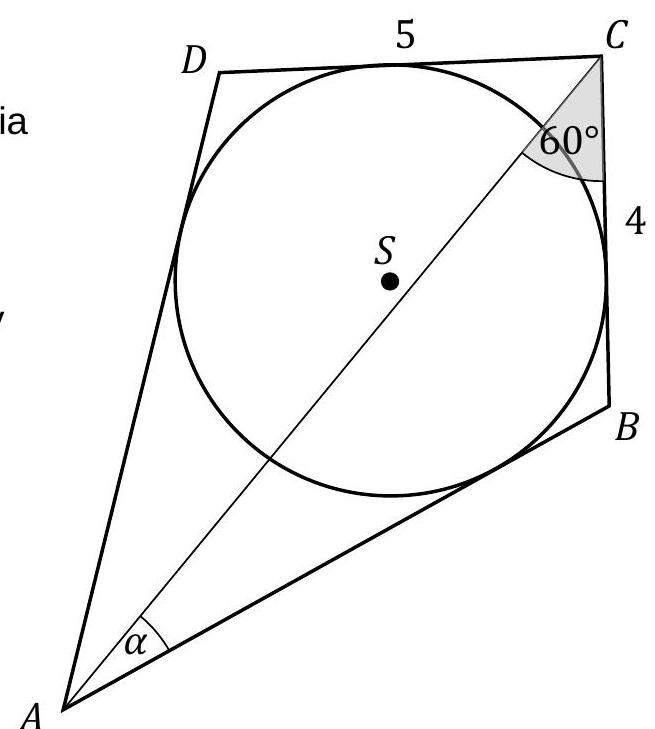
\includegraphics[max width=\textwidth, center]{2025_02_07_dcb3d059df06a3930b0ag-30}

Ponieważ w czworokąt $A B C D$ można wpisać okrąg, więc prawdziwa jest zależność

$$
|A B|+|C D|=|B C|+|A D|
$$

Zatem obwód $O b_{A B C D}$ czworokąta jest równy

$$
O b_{A B C D}=2 \cdot(|A B|+|C D|)=16 \sqrt{3}+10
$$

\section*{Sposób II}
Zauważmy, że pole trójkąta $A B C$ można obliczyć na dwa sposoby:

$$
\begin{gathered}
P=\frac{1}{2} \cdot|B C| \cdot|A C| \cdot \sin 60^{\circ}=\frac{1}{2} \cdot 4 \cdot|A C| \cdot \frac{\sqrt{3}}{2} \\
P=\frac{1}{2} \cdot|A C| \cdot|A B| \cdot \frac{1}{4}
\end{gathered}
$$

Stąd $|A B|=8 \sqrt{3}$.\\
Ponieważ w czworokąt $A B C D$ można wpisać okrąg, więc prawdziwa jest zależność

$$
|A B|+|C D|=|B C|+|A D|
$$

Zatem obwód $O b_{A B C D}$ czworokąta jest równy

$$
O b_{A B C D}=2 \cdot(|A B|+|C D|)=16 \sqrt{3}+10
$$

Sposób III\\
Oznaczmy $\alpha=|\Varangle B A C|$. Zgodnie z warunkami zadania $\sin \alpha=\frac{1}{4}$. Obliczamy długość $a$ boku $A B$.\\
Prowadzimy wysokość $B E$ trójkąta $A B C$.\\
Trójkąt prostokątny $B C E$ ma kąty ostre $30^{\circ}$ i $60^{\circ}$, więc jest „połową" trójkąta równobocznego o boku długości 4. Zatem\\
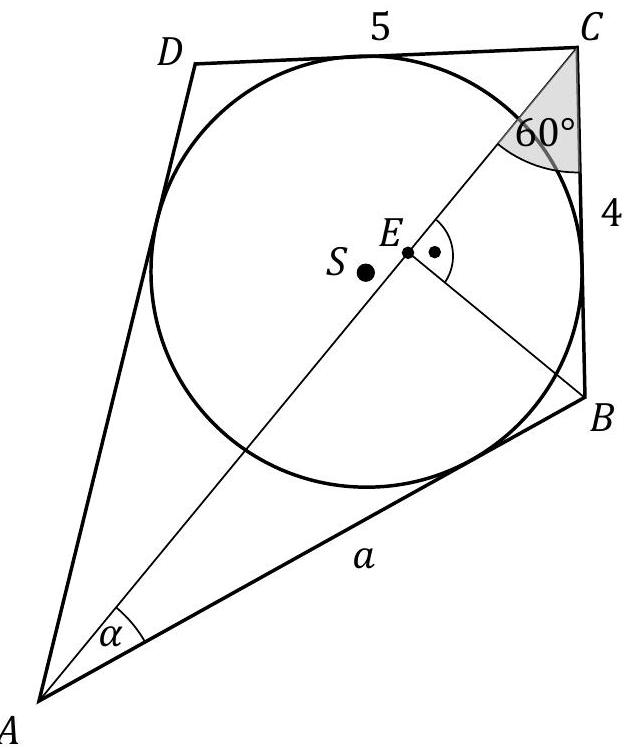
\includegraphics[max width=\textwidth, center]{2025_02_07_dcb3d059df06a3930b0ag-30(1)}

$$
|E B|=\frac{4 \sqrt{3}}{2}=2 \sqrt{3}
$$

Z definicji sinusa w trójkącie prostokątnym $A B E$ otrzymujemy

$$
\sin \alpha=\frac{|E B|}{|A B|}
$$

czyli

$$
\frac{1}{4}=\frac{2 \sqrt{3}}{|A B|}
$$

Stąd $|A B|=8 \sqrt{3}$.\\
Czworokąt $A B C D$ jest opisany na okręgu, więc $|A B|+|C D|=|B C|+|A D|$.\\
Zatem obwód $O b_{A B C D}$ czworokąta jest równy

$$
O b_{A B C D}=2 \cdot(|A B|+|C D|)=16 \sqrt{3}+10
$$

Zadanie 14. (0-4)

\begin{center}
\begin{tabular}{|l|l|}
\hline
\multicolumn{2}{|c|}{Wymagania egzaminacyjne 2023 i 2024} \\
\hline
\multicolumn{1}{|c|}{Wymaganie ogólne} & \multicolumn{1}{c|}{Wymagania szczegółowe} \\
\hline
IV. Użycie i tworzenie strategii. & Zdający: \\
 & P9.1) rozpoznaje w graniastosłupach kąty \\
 & między odcinkami (np. krawędziami, \\
 & krawędziami i przekątnymi, itp.), oblicza \\
 & miary tych kąów; \\
 & P9.3) stosuje trygonometrię do obliczeń \\
 & długości odcinków, miar kątów, pól \\
 & powierzchni i objętości graniastosłupów. \\
\hline
\end{tabular}
\end{center}

\section*{Zasady oceniania}
4 pkt - zastosowanie poprawnej metody i poprawny wynik: $\sqrt{6}$.\\
3 pkt - zapisanie równania z jedną niewiadomą (długością odcinka $S P$ ), np.:\\
$\frac{|S P|}{6}=\frac{3 \sqrt{2}}{6 \sqrt{3}}$ (z podobieństwa trójkątów PHS i $A H B$, sposób I),\\
$18 \sqrt{2}=\frac{1}{2} \cdot 3 \sqrt{2} \cdot 6+\frac{1}{2} \cdot 6 \sqrt{3} \cdot|S P|$ (z równości pól $P_{H A B}=P_{B A S}+P_{H S B}$ ),\\
$9 \sqrt{2}=\frac{1}{2} \cdot 6 \sqrt{3} \cdot|S P|$ (z równości $P_{H S B}=\frac{1}{2} \cdot|H S| \cdot|A B|=\frac{1}{2} \cdot|H B| \cdot|S P|$,\\
sposób II),\\
ALBO

\begin{itemize}
  \item obliczenie pola trójkąta $H S R$ oraz długości odcinka $H R: P_{\triangle H S R}=\frac{9 \sqrt{2}}{2}$ oraz $|H R|=3 \sqrt{3}$,\\
ALBO
  \item obliczenie długości odcinków $H P$ i $H S:|H P|=2 \sqrt{3}$ i $|H S|=3 \sqrt{2}$, ALBO
  \item obliczenie długości odcinków $H P$ oraz cosinusa/tangensa kąta $S H P:|H P|=2 \sqrt{3}$ i $\cos \Varangle S H P=\frac{\sqrt{6}}{3}\left(\operatorname{tg} \Varangle S H P=\frac{\sqrt{2}}{2}\right)$,\\
ALBO
  \item obliczenie długości $A K$ : $A K=2 \sqrt{6}$.
\end{itemize}

2 pkt - obliczenie długości boków trójkąta $H S B:|H S|=3 \sqrt{2},|H B|=6 \sqrt{3},|S B|=3 \sqrt{6}$ ALBO

\begin{itemize}
  \item zapisanie proporcji wynikającej z podobieństwa dwóch trójkątów prostokątnych, przy czym jednym z nich jest trójkąt $H S P$,\\
ALBO
  \item obliczenie/zapisanie długości odcinków $B H$ oraz $S R:|B H|=6 \sqrt{3}$ oraz $|S R|=3$, ALBO
  \item obliczenie wartości funkcji trygonometrycznej kąta $S H R$ : np. $\cos \Varangle S H R=\frac{\sqrt{6}}{3}$, $\sin \Varangle S H R=\frac{\sqrt{3}}{3}, \operatorname{tg} \Varangle S H R=\frac{\sqrt{2}}{2}$,
\end{itemize}

\section*{ALBO}
\begin{itemize}
  \item obliczenie pola trójkąta $H A B: P_{\triangle H A B}=18 \sqrt{2}$,
\end{itemize}

ALBO

\begin{itemize}
  \item obliczenie długości odcinka $S B$ i $\operatorname{sinusa}$ kąta $S B H:|S B|=3 \sqrt{6}$ i $\sin \Varangle S B H=\frac{1}{3}$, ALBO
  \item zapisanie pola trójkąta $H A B$ jako sumy pól trójkątów $S A B$ oraz $H S B$ i zapisanie $P_{H S B}=\frac{1}{2} \cdot|H B| \cdot|S P|$ (lub $P_{H S B}=\frac{1}{2} \cdot P_{H A B}$ ),\\
ALBO
  \item zapisanie pola trójkąta $H S B$ na dwa sposoby: $P_{H S B}=\frac{1}{2} \cdot|H S| \cdot|A B|$ oraz\\
$P_{H S B}=\frac{1}{2} \cdot|H B| \cdot|S P|$,\\
ALBO
  \item obliczenie pola trójkąta $H S B$ : $P_{H S B}=9 \sqrt{2}$.
\end{itemize}

1 pkt - obliczenie/zapisanie długości jednego z odcinków $B H, S R, H S$ albo $B S$ :\\
$|B H|=6 \sqrt{3},|S R|=3,|H S|=3 \sqrt{2},|B S|=3 \sqrt{6}$.\\
0 pkt - rozwiązanie, w którym zastosowano niepoprawną metodę, albo brak rozwiązania.

\section*{Uwagi:}
\begin{enumerate}
  \item Jeżeli jedynym błędem zdającego jest:\\
a) zastosowanie niepoprawnej definicji jednej funkcji trygonometrycznej\\
b) błędne zastosowanie twierdzenia Pitagorasa\\
c) zastosowanie niepoprawnej tożsamości $\sqrt{x^{2}+y^{2}}=x+y$\\
d) błędne zastosowanie twierdzenia cosinusów lub sinusów\\
e) błędne zastosowanie wzoru Herona\\
to zdający może otrzymać co najwyżej 2 punkty za całe rozwiązanie.
  \item Jeżeli zdający korzysta ze związku $|H P|=\frac{1}{3} \cdot|H B|$ (gdzie $P$ jest spodkiem wysokości poprowadzonej z wierzchołka $S$ na podstawę $H B$ trójkąta $H S B$ ) i nie uzasadni jego prawdziwości, to może otrzymać co najwyżej 2 punkty za całe rozwiązanie.
\end{enumerate}

\section*{Przykładowe pełne rozwiązania}
Przyjmijmy oznaczenia jak na rysunku:\\
$S$ - środek odcinka $A H$,\\
$R$ - środek odcinka $B H$,\\
$P$ - spodek wysokości trójkąta $S B H$ poprowadzonej z punktu $S$ na bok $B H$.\\
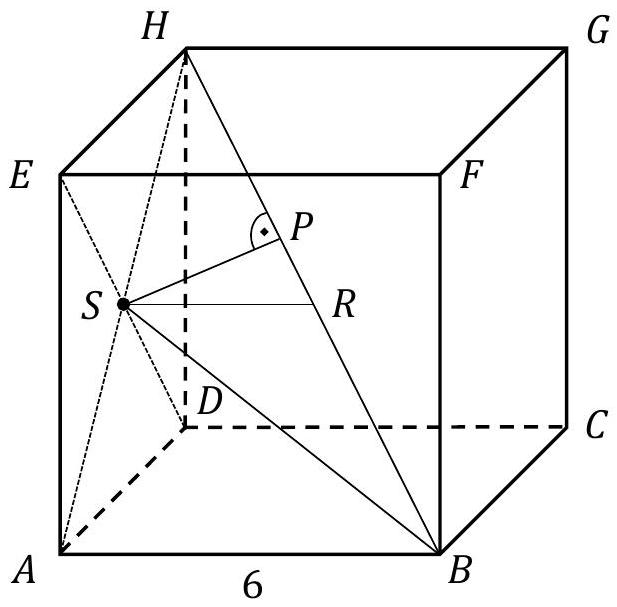
\includegraphics[max width=\textwidth, center]{2025_02_07_dcb3d059df06a3930b0ag-33}

\section*{Sposób 1}
Obliczamy $|A H|=6 \sqrt{2},|B H|=6 \sqrt{3}$.\\
Trójkąty $A H B$ i $P H S$ są podobne (cecha kkk), więc

$$
\begin{gathered}
\frac{|S P|}{|A B|}=\frac{|S H|}{|B H|} \\
\frac{|S P|}{6}=\frac{3 \sqrt{2}}{6 \sqrt{3}} \\
|S P|=\sqrt{6}
\end{gathered}
$$

\begin{center}
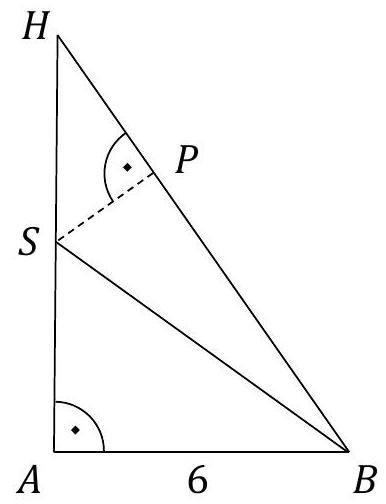
\includegraphics[max width=\textwidth]{2025_02_07_dcb3d059df06a3930b0ag-34}
\end{center}

\section*{Uwaga:}
Równanie $\frac{|S P|}{6}=\frac{3 \sqrt{2}}{6 \sqrt{3}}$ otrzymamy, stosując dwukrotnie definicję sinusa kąta $S H P$ w trójkątach prostokątnych $H S P$ i $H A B$.

\section*{Sposób II}
Obliczamy $|A H|=6 \sqrt{2},|B H|=6 \sqrt{3},|H S|=3 \sqrt{2}$.\\
Obliczamy pole trójkąta $H S B$ :\\
$P_{\triangle H S B}=\frac{1}{2} \cdot|H S| \cdot|A B|=\frac{1}{2} \cdot 3 \sqrt{2} \cdot 6=9 \sqrt{2}$\\
Ale\\
$P_{\triangle H S B}=\frac{1}{2} \cdot|H B| \cdot|S P|=\frac{1}{2} \cdot 6 \sqrt{3} \cdot|S P|=3 \sqrt{3} \cdot|S P|$\\
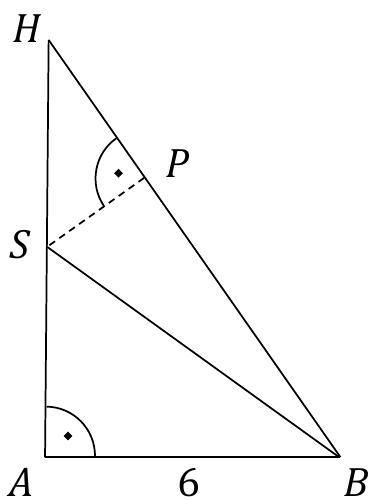
\includegraphics[max width=\textwidth, center]{2025_02_07_dcb3d059df06a3930b0ag-34(2)}

Stąd\\
$3 \sqrt{3} \cdot|S P|=9 \sqrt{2}$\\
więc $|S P|=\sqrt{6}$.\\
Sposób Ila\\
Odcinek $S R$ łączy środki boków w trójkącie $A B H$, jest więc równoległy do boku $A B$ i ma długość równą $|S R|=\frac{1}{2} \cdot 6=3$.\\
Zauważmy, że trójkąt $H A B$ jest prostokątny, zatem trójkąt $H S R$ też jest prostokątny.\\
Obliczamy $|A H|=6 \sqrt{2},|B H|=6 \sqrt{3}$.\\
Obliczamy pole trójkąta $H S R$ :\\
$P_{\triangle H S R}=\frac{1}{2}|H S| \cdot|S R|=\frac{1}{2} \cdot 3 \sqrt{2} \cdot 3=\frac{9 \sqrt{2}}{2}$\\
Ale\\
$P_{\Delta H S R}=\frac{1}{2}|H R| \cdot|S P|=\frac{1}{2} \cdot 3 \sqrt{3} \cdot|S P|$\\
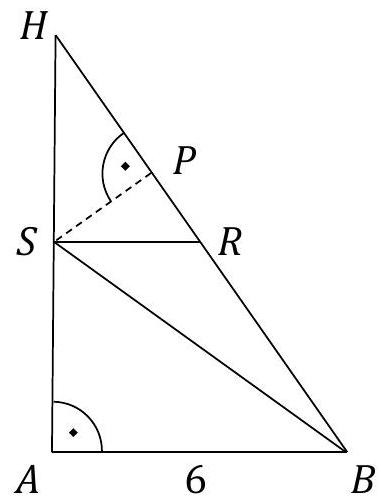
\includegraphics[max width=\textwidth, center]{2025_02_07_dcb3d059df06a3930b0ag-34(1)}

Stąd\\
$\frac{1}{2} \cdot 3 \sqrt{3} \cdot|S P|=\frac{9 \sqrt{2}}{2}$\\
więc $|S P|=\sqrt{6}$.

\section*{Sposób III}
Wyznaczamy cosinus kąta SHP:\\
$\cos \Varangle S H P=\frac{|A H|}{|B H|}=\frac{6 \sqrt{2}}{6 \sqrt{3}}=\frac{\sqrt{6}}{3}$\\
Ponieważ $\cos \Varangle S H P=\frac{|H P|}{|H S|}=\frac{|H P|}{3 \sqrt{2}}$, więc $\frac{|H P|}{3 \sqrt{2}}=\frac{\sqrt{6}}{3}$ i stąd $|H P|=2 \sqrt{3}$.\\
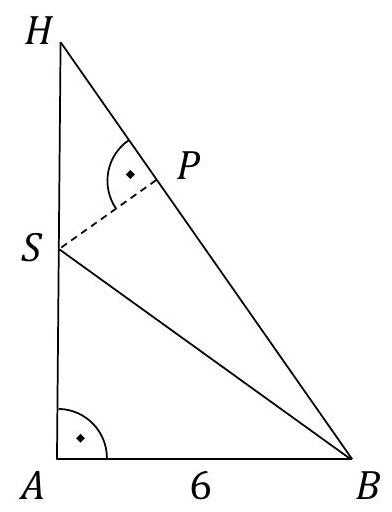
\includegraphics[max width=\textwidth, center]{2025_02_07_dcb3d059df06a3930b0ag-35(1)}

Z twierdzenia Pitagorasa w trójkącie HPS mamy $(3 \sqrt{2})^{2}=|S P|^{2}+(2 \sqrt{3})^{2}$, więc $|S P|=\sqrt{6}$.

\section*{Sposób IV}
Obliczamy $|A H|=6 \sqrt{2},|B H|=6 \sqrt{3}$.\\
Zauważamy, że trójkąt $H A B$ jest prostokątny. Pole trójkąta $H A B$ jest równe

$$
P_{\triangle H A B}=\frac{6 \sqrt{2} \cdot 6}{2}=18 \sqrt{2}
$$

Niech punkt $K$ będzie rzutem wierzchołka $A$ na bok $B H$ trójkąta $H A B$, zatem

$$
\begin{gathered}
\frac{|A K| \cdot|H B|}{2}=18 \sqrt{2} \\
|A K|=\frac{36 \sqrt{2}}{|H B|}=\frac{36 \sqrt{2}}{6 \sqrt{3}}=2 \sqrt{6}
\end{gathered}
$$

Ponieważ trójkąty $H S P$ i $H A K$ są podobne, więc

$$
\frac{|H S|}{|S P|}=\frac{|H A|}{|A K|}
$$

Stąd

$$
|S P|=\frac{3 \sqrt{2} \cdot 2 \sqrt{6}}{6 \sqrt{2}}=\sqrt{6}
$$

\begin{center}
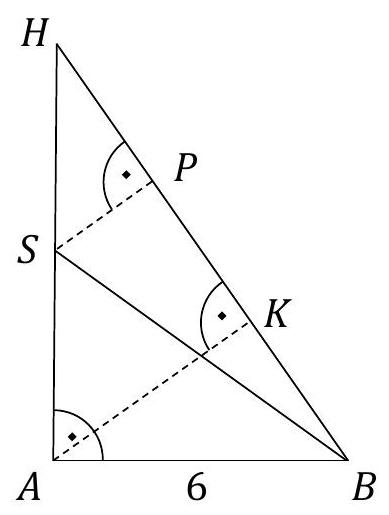
\includegraphics[max width=\textwidth]{2025_02_07_dcb3d059df06a3930b0ag-35}
\end{center}

\section*{Uwaga:}
Zadanie można również rozwiązać, rozważając ostrosłupy $D E G H$ oraz $D E G B$.\\
Prowadzimy odcinki $E G$ i $D G$. Trójkąt $E D G$ jest równoboczny, gdyż wszystkie jego boki są przekątnymi przystających kwadratów, a ponieważ odcinki $D H, E H$ i $G H$ mają równe długości, odcinki $D B, E B$ i $G B$ też mają równe długości, więc ostrosłupy $D E G H$ i $D E G B$ o wspólnej podstawie $D E G$ są prawidłowe.\\
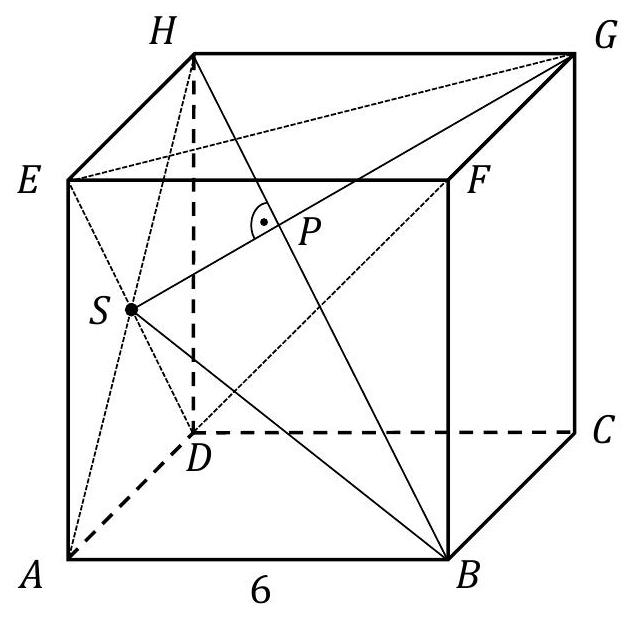
\includegraphics[max width=\textwidth, center]{2025_02_07_dcb3d059df06a3930b0ag-36}

Wynika stąd, że prosta $B H$ zawiera wysokości tych ostrosłupów, a to oznacza, że punkt $P$ jest środkiem ciężkości trójkąta $D E G$ o boku długości $|D E|=6 \sqrt{2}$. Zatem

$$
|S P|=\frac{1}{3} \cdot \frac{6 \sqrt{2} \cdot \sqrt{3}}{2}=\sqrt{6}
$$

Zadanie 15. (0-5)

\begin{center}
\begin{tabular}{|l|l|}
\hline
\multicolumn{2}{|c|}{Wymagania egzaminacyjne 2023 i 2024} \\
\hline
\multicolumn{1}{|c|}{Wymaganie ogólne} & \multicolumn{1}{|c|}{Wymagania szczegółowe} \\
\hline
III. Modelowanie matematyczne. & Zdajacy: \\
 & R3.1) stosuje wzory Viète'a; \\
 & R3.2) rozwiązuje równania i nierówności \\
 & liniowe i kwadratowe z parametrem. \\
\hline
\end{tabular}
\end{center}

\section*{Zasady oceniania}
Rozwiązanie zadania składa się z trzech etapów.\\
Pierwszy etap polega na rozwiązaniu nierówności $\Delta>0$. Za poprawne wykonanie tego etapu zdający otrzymuje 1 punkt.\\
1 pkt - poprawne rozwiązanie nierówności $\Delta>0: m \in(-\infty, 2) \cup\left(\frac{11}{5},+\infty\right)$.\\
0 pkt - rozwiązanie, w którym zastosowano niepoprawną metodę, albo brak rozwiązania.

\section*{Uwaga:}
Jeżeli zdający rozwiązuje warunek $\Delta \geq 0$, to za tę część rozwiązania otrzymuje 0 punktów.\\
Drugi etap polega na wyznaczeniu tych wartości parametru $m$, dla których jest spełniony warunek $x_{1}^{3}+x_{2}^{3}>-28$. Za poprawne wykonanie tego etapu zdający otrzymuje 3 punkty. Podział punktów za drugi etap rozwiązania:\\
3 pkt - rozwiązanie nierówności z jedną niewiadomą $m$, wynikającej $z$ warunku

$$
x_{1}^{3}+x_{2}^{3}>-28: m \in\left(2, \frac{9}{4}\right) .
$$

2 pkt - zapisanie nierówności z jedną niewiadomą $m$, wynikającej $z$ warunku

$$
x_{1}^{3}+x_{2}^{3}>-28, \text { np. }-64-3 \cdot\left(-\frac{m-3}{m-2}\right) \cdot(-4)>-28
$$

ALBO

\begin{itemize}
  \item zapisanie nierówności $\left(-2-\sqrt{\frac{5 m-11}{m-2}}\right)^{3}+\left(-2+\sqrt{\frac{5 m-11}{m-2}}\right)^{3}>-28$ i poprawne zastosowanie wzoru skróconego mnożenia na sześcian sumy/różnicy do co najmniej jednego ze składników sumy $\left(-2-\sqrt{\frac{5 m-11}{m-2}}\right)^{3}+\left(-2+\sqrt{\frac{5 m-11}{m-2}}\right)^{3}$.\\
1 pkt - przekształcenie nierówności $x_{1}^{3}+x_{2}^{3}>-28$ do postaci pozwalającej na\\
bezpośrednie zastosowanie wzorów Viète'a, np.\\
$\left(x_{1}+x_{2}\right)^{3}-3 x_{1} x_{2}\left(x_{1}+x_{2}\right)>-28$\\
ALBO
  \item wyznaczenie pierwiastków trójmianu kwadratowego $x^{2}+4 x-\frac{m-3}{m-2}$ w zależności\\
od $m: x_{1}=\frac{-4-\sqrt{\frac{20 m-44}{m-2}}}{2 \cdot 1}, x_{2}=\frac{-4+\sqrt{\frac{20 m-44}{m-2}}}{2 \cdot 1}$.\\
0 pkt - rozwiązanie, w którym zastosowano niepoprawną metodę, albo brak rozwiązania.
\end{itemize}

Trzeci etap polega na wyznaczeniu wszystkich wartości parametru $m$, które spełniają jednocześnie dwa warunki: $\Delta>0$ i $x_{1}^{3}+x_{2}^{3}>-28: m \in\left(\frac{11}{5}, \frac{9}{4}\right)$.\\
Za poprawne wykonanie tego etapu zdający otrzymuje 1 punkt.\\
1 pkt - poprawne wyznaczenie wszystkich wartości parametru $m$, które spełniają jednocześnie warunki $\Delta>0$ i $x_{1}^{3}+x_{2}^{3}>-28: m \in\left(\frac{11}{5}, \frac{9}{4}\right)$.\\
0 pkt - rozwiązanie, w którym zastosowano niepoprawną metodę, albo brak rozwiązania.

\section*{Uwagi:}
\begin{enumerate}
  \item Jeżeli zdający popełni w I i/lub II etapie jedynie błędy rachunkowe i otrzyma zbiory rozwiązań z li ll etapu, które nie są rozłączne i żaden z nich nie jest zbiorem liczb rzeczywistych, a następnie poprawnie wyznaczy część wspólną zbiorów rozwiązań z etapów I i II, to za III etap otrzymuje 1 punkt.
  \item Jeżeli zdający w II etapie rozwiązania popełni błąd i przyjmie, że $x_{1}+x_{2}= \pm \frac{m-3}{m-2}$ lub $x_{1} \cdot x_{2}= \pm 4$, to za II etap może otrzymać co najwyżej 1 punkt, a za III etap otrzymuje 0 punktów.
  \item Jeżeli zdający w II etapie rozwiązania popełni błąd, który nie jest rachunkowy (np. pominie istotne nawiasy przy przekształcaniu nierówności $x_{1}^{3}+x_{2}^{3}>-28$ do postaci pozwalającej na bezpośrednie zastosowanie wzorów Viète’a, albo przyjmie, że $x_{1}^{3}+x_{2}^{3}=\left(x_{1}+x_{2}\right)\left[\left(x_{1}+x_{2}\right)^{2}-x_{1} \cdot x_{2}\right]$, i konsekwentnie do popełnionego błędu doprowadzi rozwiązanie II etapu zadania do końca, to może uzyskać co najwyżej 1 punkt za II etap.
\end{enumerate}

\section*{Przykładowe pełne rozwiązanie}
\section*{I etap}
Trójmian kwadratowy $x^{2}+4 x-\frac{m-3}{m-2}$, gdzie $m \neq 2$, ma dwa różne pierwiastki rzeczywiste wtedy i tylko wtedy, gdy wyróżnik tego trójmianu jest dodatni. Rozwiązujemy warunek $\Delta>0$ :

$$
\begin{gathered}
4^{2}-4 \cdot\left(-\frac{m-3}{m-2}\right)>0 \\
\frac{20 m-44}{m-2}>0 \\
(20 m-44) \cdot(m-2)>0 \\
20\left(m-\frac{11}{5}\right) \cdot(m-2)>0 \\
m \in(-\infty, 2) \cup\left(\frac{11}{5},+\infty\right)
\end{gathered}
$$

\section*{II etap}
\section*{Sposób 1}
Wyznaczamy wszystkie wartości parametru $m \neq 2$, dla których jest spełniony warunek $x_{1}^{3}+x_{2}^{3}>-28$, korzystając ze wzorów Viète'a:

$$
\begin{gathered}
\left(x_{1}+x_{2}\right)^{3}-3 x_{1} x_{2}\left(x_{1}+x_{2}\right)>-28 \\
-64-3 \cdot\left(-\frac{m-3}{m-2}\right) \cdot(-4)>-28 \\
\frac{m-3}{m-2}<-3 \\
(4 m-9)(m-2)<0 \\
m \in\left(2, \frac{9}{4}\right)
\end{gathered}
$$

\section*{Sposób II}
Wyznaczamy pierwiastki $x_{1}$, $x_{2}$ trójmianu kwadratowego $x^{2}+4 x-\frac{m-3}{m-2}$ :

$$
\begin{aligned}
& x_{1}=\frac{-4-\sqrt{\frac{20 m-44}{m-2}}}{2 \cdot 1}=-2-\sqrt{\frac{5 m-11}{m-2}} \\
& x_{2}=\frac{-4+\sqrt{\frac{20 m-44}{m-2}}}{2 \cdot 1}=-2+\sqrt{\frac{5 m-11}{m-2}}
\end{aligned}
$$

Nierówność $x_{1}^{3}+x_{2}^{3}>-28$ możemy więc zapisać w postaci

$$
\left(-2-\sqrt{\frac{5 m-11}{m-2}}\right)^{3}+\left(-2+\sqrt{\frac{5 m-11}{m-2}}\right)^{3}>-28
$$

Oznaczmy $\sqrt{\frac{5 m-11}{m-2}}$ przez $p$. Wtedy

$$
(-2-p)^{3}+(-2+p)^{3}>-28
$$

Korzystając ze wzoru na sześcian różnicy i sześcian sumy, otrzymujemy dalej

$$
\begin{gathered}
\left(-8-12 p-6 p^{2}-p^{3}\right)+\left(-8+12 p-6 p^{2}+p^{3}\right)>-28 \\
-12 p^{2}-16>-28 \\
12 p^{2}-12<0 \\
p^{2}-1<0
\end{gathered}
$$

Zatem

$$
\begin{gathered}
\left(\sqrt{\frac{5 m-11}{m-2}}\right)^{2}-1<0 \\
\frac{5 m-11}{m-2}-1<0
\end{gathered}
$$

$$
\begin{gathered}
\frac{5 m-11-m+2}{m-2}<0 \\
\frac{4 m-9}{m-2}<0 \\
(4 m-9)(m-2)<0 \\
m \in\left(2, \frac{9}{4}\right)
\end{gathered}
$$

\section*{Uwaga:}
Nierówność $(-2-p)^{3}+(-2+p)^{3}>-28$ możemy również przekształcić, korzystając ze wzoru na sumę sześcianów. Wtedy otrzymujemy

$$
\begin{gathered}
(-2-p+(-2)+p)\left[(-2-p)^{2}-(-2-p)(-2+p)+(-2+p)^{2}\right]>-28 \\
-4\left(4+4 p+p^{2}+p^{2}-4+4-4 p+p^{2}\right)>-28 \\
3 p^{2}+4<7 \\
p^{2}-1<0
\end{gathered}
$$

\section*{III etap}
Wyznaczamy wszystkie wartości parametru $m \neq 2$, które jednocześnie spełniają warunki $m \in(-\infty, 2) \cup\left(\frac{11}{5},+\infty\right)$ oraz $m \in\left(2, \frac{9}{4}\right): m \in\left(\frac{11}{5}, \frac{9}{4}\right)$.

Zadanie 16. (0-7)

\begin{center}
\begin{tabular}{|l|l|}
\hline
\multicolumn{2}{|c|}{Wymagania egzaminacyjne 2023 i 2024} \\
\hline
\multicolumn{1}{|c|}{Wymaganie ogólne} & \multicolumn{1}{c|}{Wymaganie szczegółowe} \\
\hline
III. Modelowanie matematyczne. & \begin{tabular}{l}
Zdający: \\
 \\
 \\
 \\
 \\
 \\
 \\
 \\
R11.6) stosuje pochodne do rozwiązywania optymalizacyjnych. \\
\hline
\end{tabular} \\
\hline
\end{tabular}
\end{center}

\section*{Zasady oceniania}
\section*{Część a)}
3 pkt - wyznaczenie pola $P$ trójkąta $A B C$ jako funkcji zmiennej $m: P(m)=\frac{m^{2}}{m-4}$.\\
2 pkt - wyznaczenie pierwszej (lub drugiej) wspórrzędnej punktu $C$ : $x_{C}=\frac{m}{4-m}$ (lub $y_{C}=\frac{2 m}{m-4}$ ).\\
1 pkt - wyznaczenie współczynnika kierunkowego prostej $B D: \frac{2}{3-m}$\\
ALBO

\begin{itemize}
  \item zapisanie równania prostej $B D$ w postaci ogólnej, np. $2 x+(m-3) y-2 m=0$.
\end{itemize}

0 pkt - rozwiązanie, w którym zastosowano niepoprawną metodę, albo brak rozwiązania.

\section*{Część b)}
4 pkt - wyznaczenie równania prostej $B C$ w przypadku, gdy pole trójkąta $A B C$ jest najmniejsze, np. $y=-\frac{2}{5} x+\frac{16}{5}$.\\
3 pkt - zbadanie znaku pochodnej funkcji $P: P^{\prime}(m)>0$ dla $m \in(8,+\infty)$ oraz $P^{\prime}(m)<0$ dla $m \in(4,8)$, oraz wyznaczenie (z uzasadnieniem) wartości zmiennej $m$, dla której funkcja $P$ osiąga wartość najmniejszą, np.\\
funkcja $P$ zmiennej $m$ (określona na przedziale $(4,+\infty)$ ) jest rosnąca w przedziale $\langle 8,+\infty$ ) oraz malejąca w przedziale $(4,8\rangle$, więc w punkcie $m=8$ osiąga najmniejszą wartość\\
ALBO

\begin{itemize}
  \item uzasadnienie, że dla $m=8$ funkcja $P$ osiąga wartość najmniejszą (przy metodzie średnich liczbowych).\\
2 pkt - obliczenie miejsc zerowych pochodnej funkcji $P: m=8$\\
ALBO
  \item obliczenie wartości $m$, dla której zachodzi równość średniej arytmetycznej\\
i geometrycznej liczb dodatnich $m-4$ oraz $\frac{16}{m-4}: m=8$.\\
1 pkt - wyznaczenie wzoru pochodnej funkcji $P$, np. $P^{\prime}(m)=\frac{2 m(m-4)-m^{2} \cdot 1}{(m-4)^{2}}$\\
ALBO
  \item zapisanie nierówności między średnią arytmetyczną a geometryczną liczb $m$-4 oraz $\frac{16}{m-4}$ :
\end{itemize}

$$
\frac{m-4+\frac{16}{m-4}}{2} \geq \sqrt{(m-4) \cdot \frac{16}{m-4}}
$$

ALBO

\begin{itemize}
  \item zapisanie nierówności między średnią arytmetyczną a geometryczną liczb $m-4,4$ oraz $\frac{16}{m-4}$ :
\end{itemize}

$$
\frac{m-4+4+\frac{16}{m-4}}{3} \geq \sqrt[3]{(m-4) \cdot 4 \cdot \frac{16}{m-4}}
$$

0 pkt - rozwiązanie, w którym zastosowano niepoprawną metodę, albo brak rozwiązania.

\section*{Uwagi do części b):}
\begin{enumerate}
  \item Badanie znaku pochodnej zdający może opisać w inny sposób, np. szkicując wykres funkcji, która w ten sam sposób jak pochodna zmienia znak i zaznaczając na rysunku, np. znakami „+" $i$ „-", znak pochodnej.
  \item Za poprawne uzasadnienie, że rozważana funkcja posiada wartość najmniejszą dla wyznaczonej wartości $m$, przy której pochodna się zeruje, można uznać sytuację, gdy zdający:
\end{enumerate}

\begin{itemize}
  \item opisuje (słownie lub graficznie - np. przy użyciu strzałek) monotoniczność funkcji $P$ lub
  \item zapisuje, że dla wyznaczonej wartości $m$ funkcja $P$ ma minimum lokalne ijest to jednocześnie jej najmniejsza wartość.\\
Jeżeli zdający nie przedstawi takiego uzasadnienia, to za część b) może otrzymać co najwyżej 3 punkty.
\end{itemize}

\begin{enumerate}
  \setcounter{enumi}{2}
  \item Jeżeli zdający, przy uzasadnieniu, że funkcja $P$ przyjmuje najmniejszą wartość dla $m=8$, nie ogranicza się do przedziału $(4,+\infty)$, to za część b) może otrzymać co najwyżej 3 punkty.
  \item Akceptujemy przedziały monotoniczności $(4,8),(8,+\infty)$.
  \item Jeżeli zdający wyznaczy minimum lokalne i nie zapisze, że jest to wartość najmniejsza, to otrzymuje co najwyżej 3 punkty za część b).
\end{enumerate}

\section*{Przykładowe pełne rozwiązania}
\section*{a)}
\section*{Sposób 1}
Wyznaczamy współczynnik kierunkowy prostej $B D$ : $a_{B D}=\frac{2-0}{3-m}=\frac{2}{3-m}$.\\
Prosta $B D$ ma równanie $y=\frac{2}{3-m} \cdot(x-m)$.\\
Wyznaczamy współrzędne wierzchołka $C=\left(x_{C}, y_{C}\right)$, rozwiązując układ równań\\
$y=\frac{2}{3-m} \cdot(x-m)$ i $y=-2 x$.\\
Stąd, dla $m>4$, otrzymujemy

$$
\begin{gathered}
\frac{2}{3-m} \cdot\left(x_{C}-m\right)=-2 x_{C} \\
\left(\frac{2}{3-m}+2\right) x_{C}=\frac{2 m}{3-m} \\
\frac{8-2 m}{3-m} \cdot x_{C}=\frac{2 m}{3-m} \\
\frac{4-m}{3-m} \cdot x_{C}=\frac{m}{3-m} \\
x_{C}=\frac{m}{4-m}
\end{gathered}
$$

Wtedy $y_{C}=-2 \cdot \frac{m}{4-m}=\frac{2 m}{m-4}$. Zatem $C=\left(\frac{m}{4-m}, \frac{2 m}{m-4}\right)$.\\
Podstawa $A B$ trójkąta $A B C$ ma długość $|m|$. Wysokość trójkąta $A B C$ opuszczona z wierzchołka $C$ jest równa $\left|\frac{2 m}{m-4}\right|$. Zatem pole $P$ tego trójkąta, jako funkcja zmiennej $m$, jest określone wzorem

$$
P(m)=\frac{1}{2} \cdot|m| \cdot\left|\frac{2 m}{m-4}\right|
$$

Ponieważ $m>4$, więc $P(m)=\frac{m^{2}}{m-4}$.

\section*{Sposób II}
Wyznaczamy współczynnik kierunkowy prostej $B D$ : $a_{B D}=\frac{2-0}{3-m}=\frac{2}{3-m}$.\\
Punkt $C$ leży na prostej $y=-2 x$, zatem ma wspórrzędne $\left(x_{C},-2 x_{C}\right)$.\\
Wyznaczamy współczynnik kierunkowy prostej $B C$ : $a_{B C}=\frac{-2 x_{C}-0}{x_{C}-m}=\frac{2 x_{C}}{m-x_{C}}$.\\
Ponieważ $a_{B D}=a_{B C}$, więc dla $m>4$ otrzymujemy

$$
\frac{2}{3-m}=\frac{2 x_{C}}{m-x_{C}}
$$

Stąd

$$
x_{C}=\frac{m}{4-m}
$$

Wtedy $-2 x_{C}=-2 \cdot \frac{m}{4-m}=\frac{2 m}{m-4}$. Zatem $C=\left(\frac{m}{4-m}, \frac{2 m}{m-4}\right)$.\\
Podstawa $A B$ trójkąta $A B C$ ma długość $|m|$. Wysokość trójkąta $A B C$ opuszczona z wierzchołka $C$ jest równa $\left|\frac{2 m}{m-4}\right|$. Zatem pole $P$ tego trójkąta, jako funkcja zmiennej $m$, jest określone wzorem

$$
P(m)=\frac{1}{2} \cdot|m| \cdot\left|\frac{2 m}{m-4}\right|
$$

Ponieważ $m>4$, więc $P(m)=\frac{m^{2}}{m-4}$.\\
b)

Sposób 1\\
Wyznaczamy pochodną funkcji $P$ :

$$
P^{\prime}(m)=\frac{2 m(m-4)-m^{2} \cdot 1}{(m-4)^{2}}=\frac{m^{2}-8 m}{(m-4)^{2}}=\frac{m(m-8)}{(m-4)^{2}}
$$

Obliczamy miejsca zerowe pochodnej funkcji $P$ :

$$
\begin{gathered}
P^{\prime}(m)=0 \quad \text { i } \quad m \in(4,+\infty) \\
\frac{m(m-8)}{(m-4)^{2}}=0 \quad \text { i } \quad m \in(4,+\infty) \\
m(m-8)=0 \quad \text { i } \quad m \in(4,+\infty) \\
m=8
\end{gathered}
$$

Ponieważ $P^{\prime}(m)>0$ dla $m \in(8,+\infty)$ oraz $P^{\prime}(m)<0$ dla $m \in(4,8)$, więc funkcja $P$ jest malejąca w przedziale ( 4,8$\rangle$ oraz rosnąca w przedziale $\langle 8,+\infty$ ). Zatem funkcja $P$ osiąga wartość najmniejszą dla $m=8$.\\
Gdy $m=8$, to prosta $B C$ przechodzi przez punkty $B=(8,0)$ oraz $D=(3,2)$, więc ma równanie $y=\frac{2}{3-8} \cdot(x-8)$, czyli $y=-\frac{2}{5} x+\frac{16}{5}$.

\section*{Sposób II}
Przekształcamy wyrażenie $\frac{m^{2}}{m-4}$ :

$$
\frac{m^{2}}{m-4}=\frac{\left(m^{2}-8 m+16\right)+8 m-32+16}{m-4}=(m-4)+8+\frac{16}{m-4}
$$

Ponieważ $m>4$, więc liczby $m-4$ oraz $\frac{16}{m-4}$ są dodatnie. Z nierówności między średnimi arytmetyczną i geometryczną dla liczb dodatnich $m-4$ oraz $\frac{16}{m-4}$ otrzymujemy:

$$
\begin{gathered}
\frac{m-4+\frac{16}{m-4}}{2} \geq \sqrt{(m-4) \cdot \frac{16}{m-4}} \\
\frac{m-4+\frac{16}{m-4}}{2} \geq \sqrt{16} \\
m-4+\frac{16}{m-4} \geq 8 \\
m-4+8+\frac{16}{m-4} \geq 16 \\
P(m) \geq 16
\end{gathered}
$$

przy czym równość zachodzi tylko dla tych $m$, dla których $m-4=\frac{16}{m-4}$ i jednocześnie $m>4$, tj. dla $m=8$.\\
Zatem funkcja $P$ osiąga wartość najmniejszą dla $m=8$.\\
Gdy $m=8$, to prosta $B C$ przechodzi przez punkty $B=(8,0)$ oraz $D=(3,2)$, więc ma równanie $y=\frac{2}{3-8} \cdot(x-8)$, czyli $y=-\frac{2}{5} x+\frac{16}{5}$.


\end{document}